%%%%%%%%%%%%%%
\begin{figure}[h!]
\begin{center}
\begin{tabular}{ccc}
%
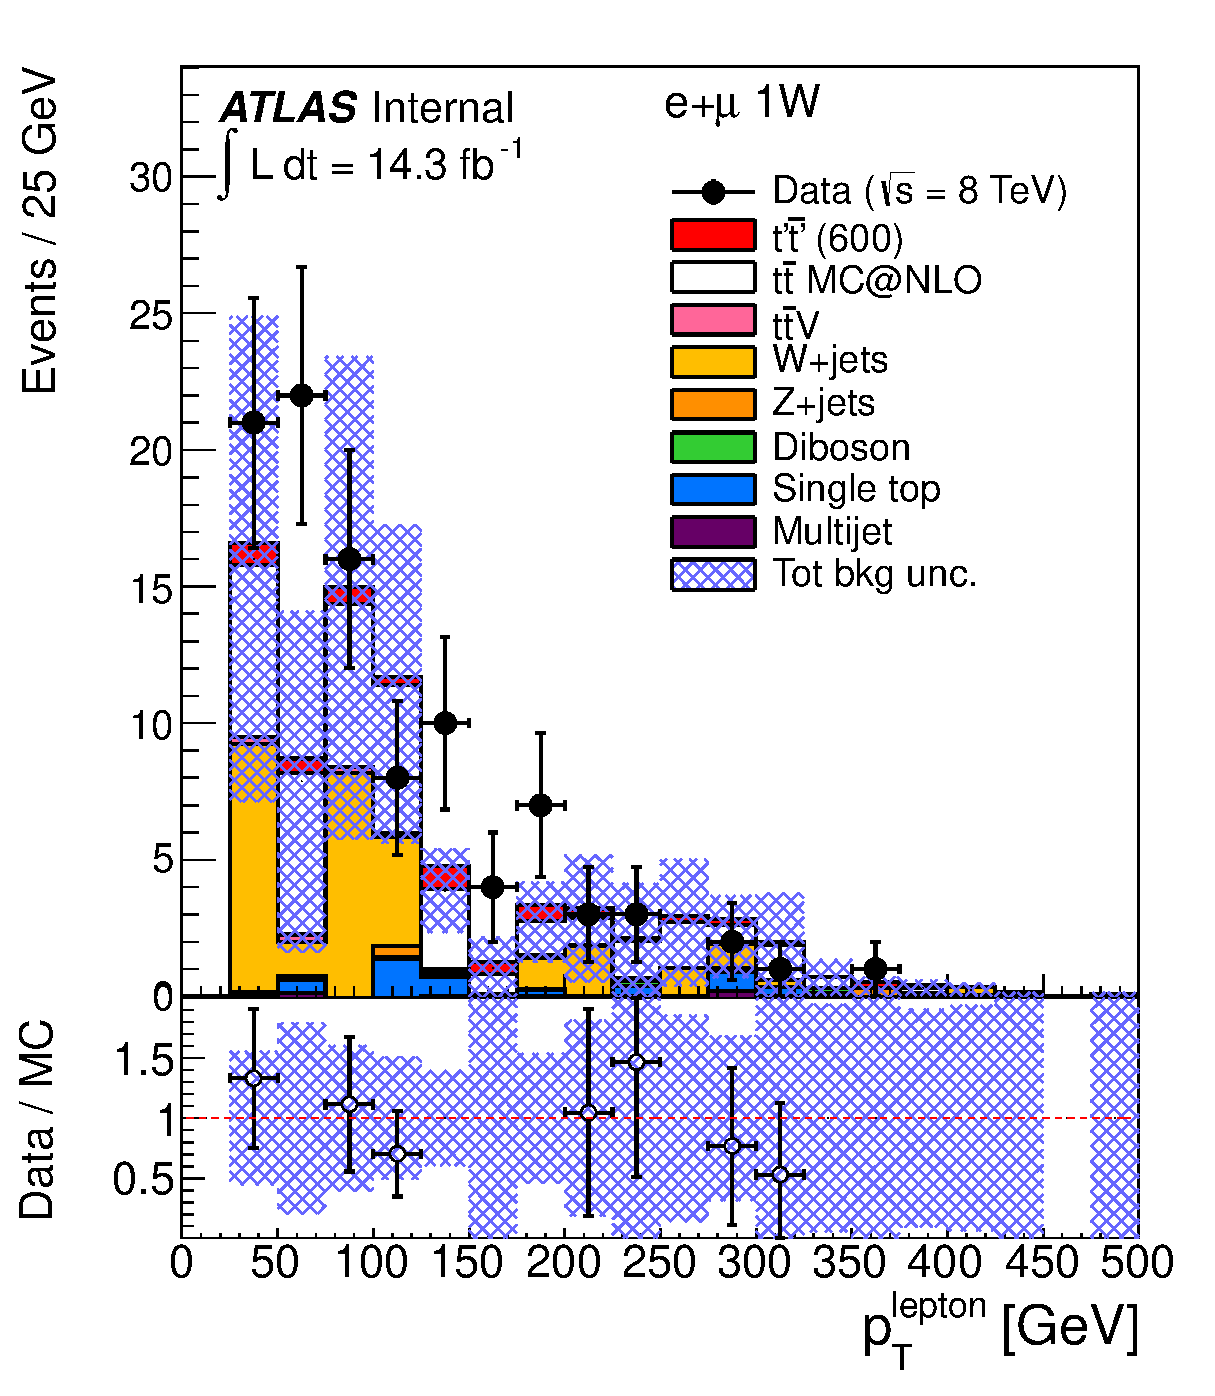
\includegraphics[width=0.30\textwidth]{appendices/figures/sdrs/LepPt_ELEMUONCR8_1W_NOMINAL.eps} &
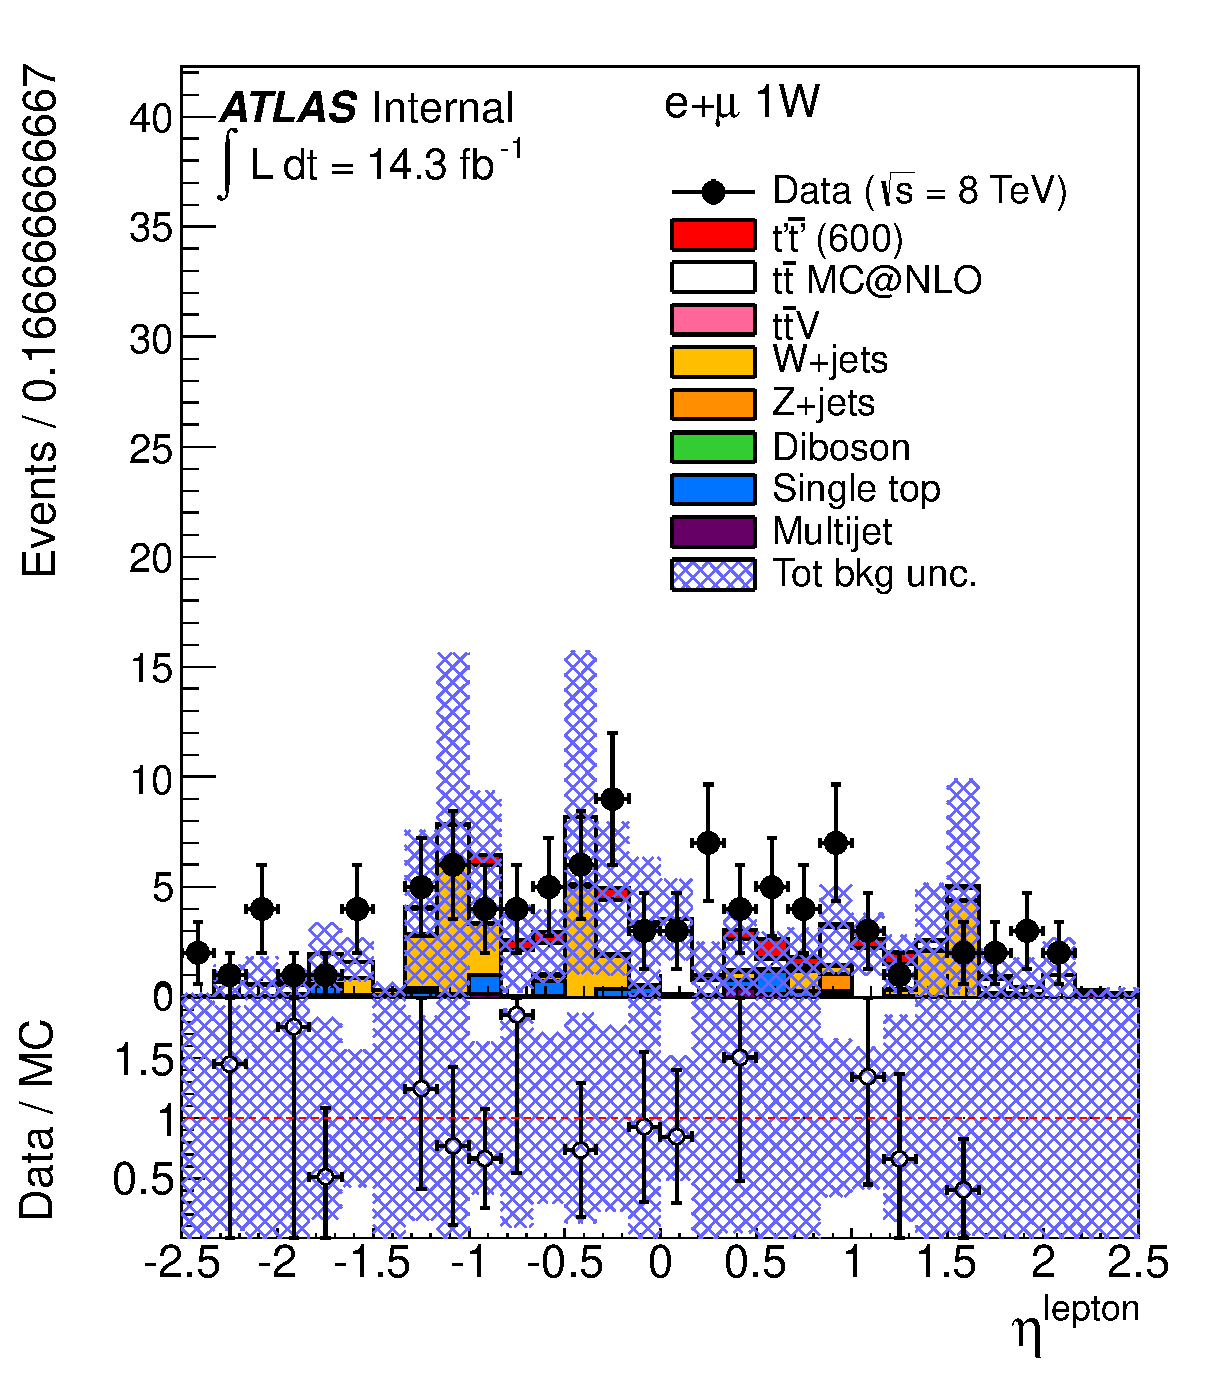
\includegraphics[width=0.30\textwidth]{appendices/figures/sdrs/LepEta_ELEMUONCR8_1W_NOMINAL.eps} &
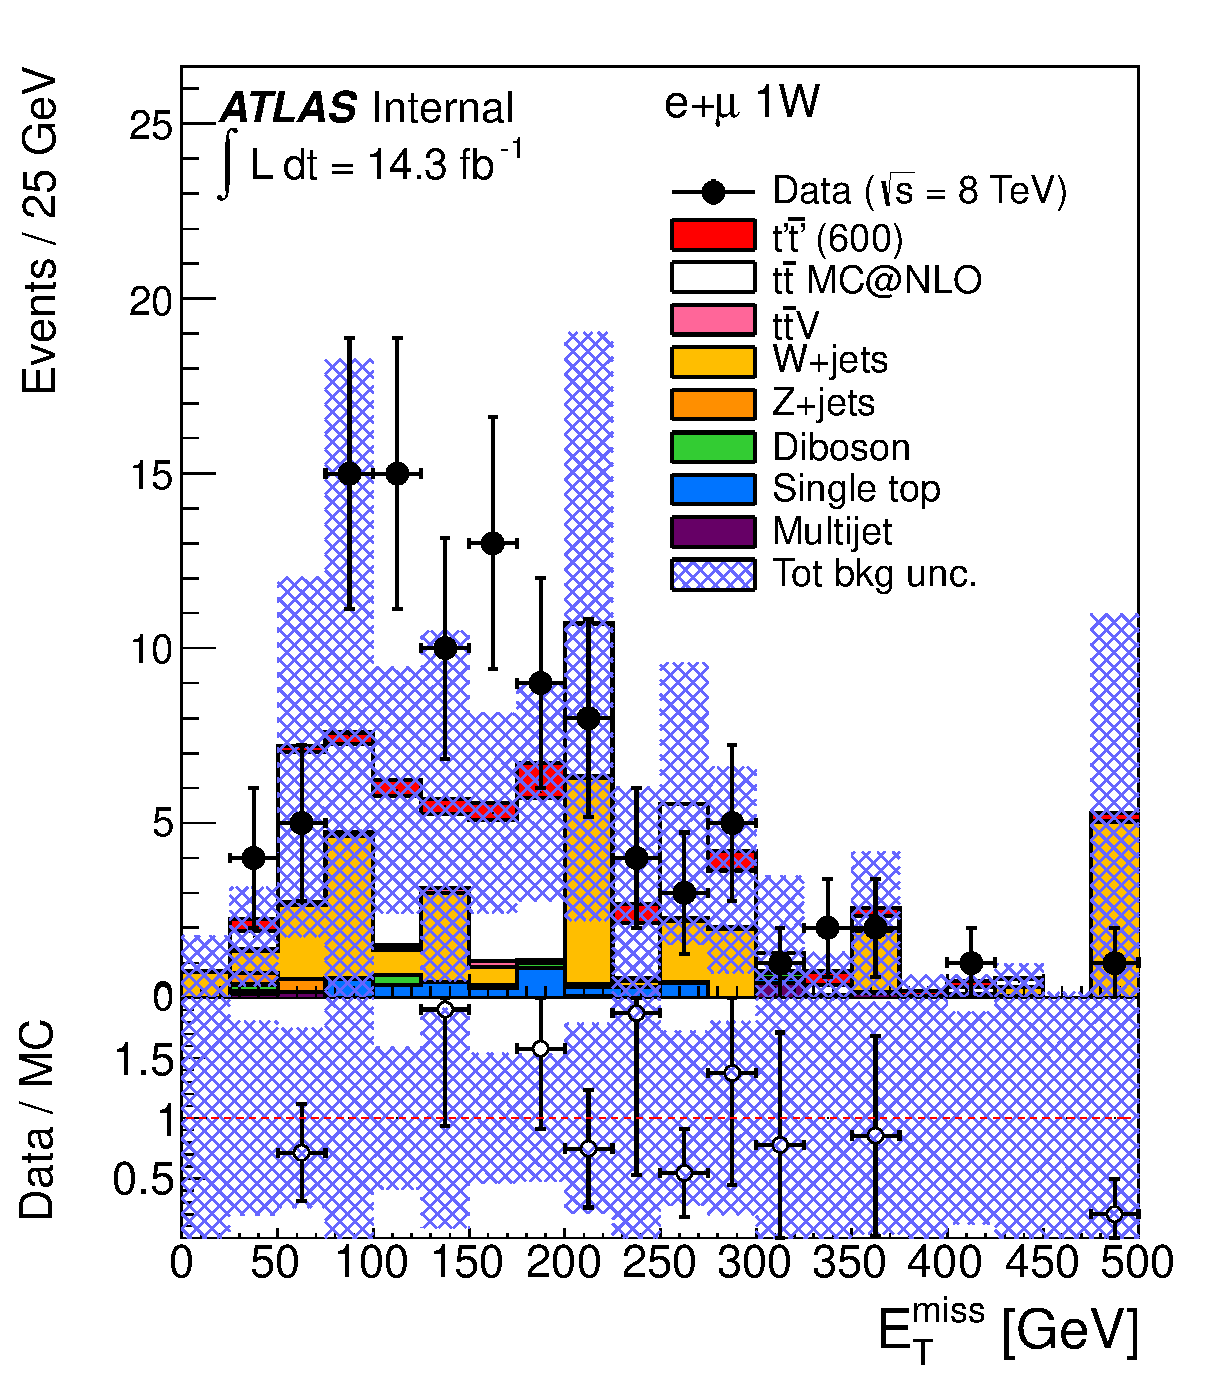
\includegraphics[width=0.30\textwidth]{appendices/figures/sdrs/MET_ELEMUONCR8_1W_NOMINAL.eps} \\
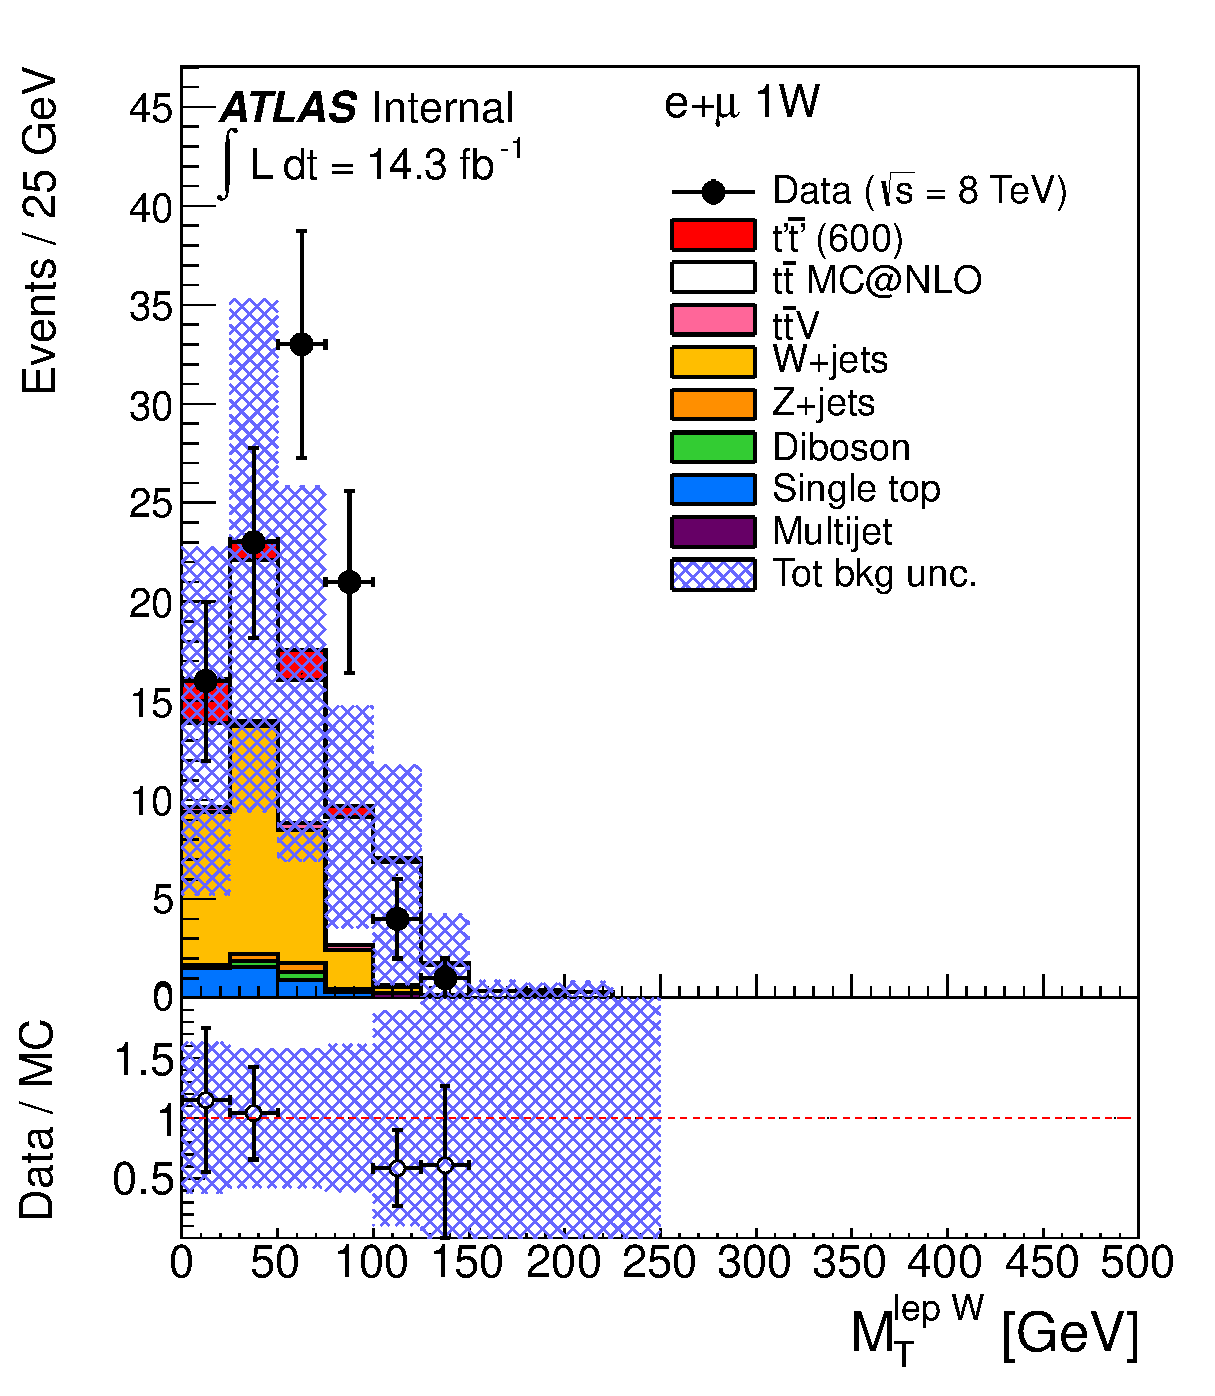
\includegraphics[width=0.30\textwidth]{appendices/figures/sdrs/Wlep_MassT_ELEMUONCR8_1W_NOMINAL.eps} &
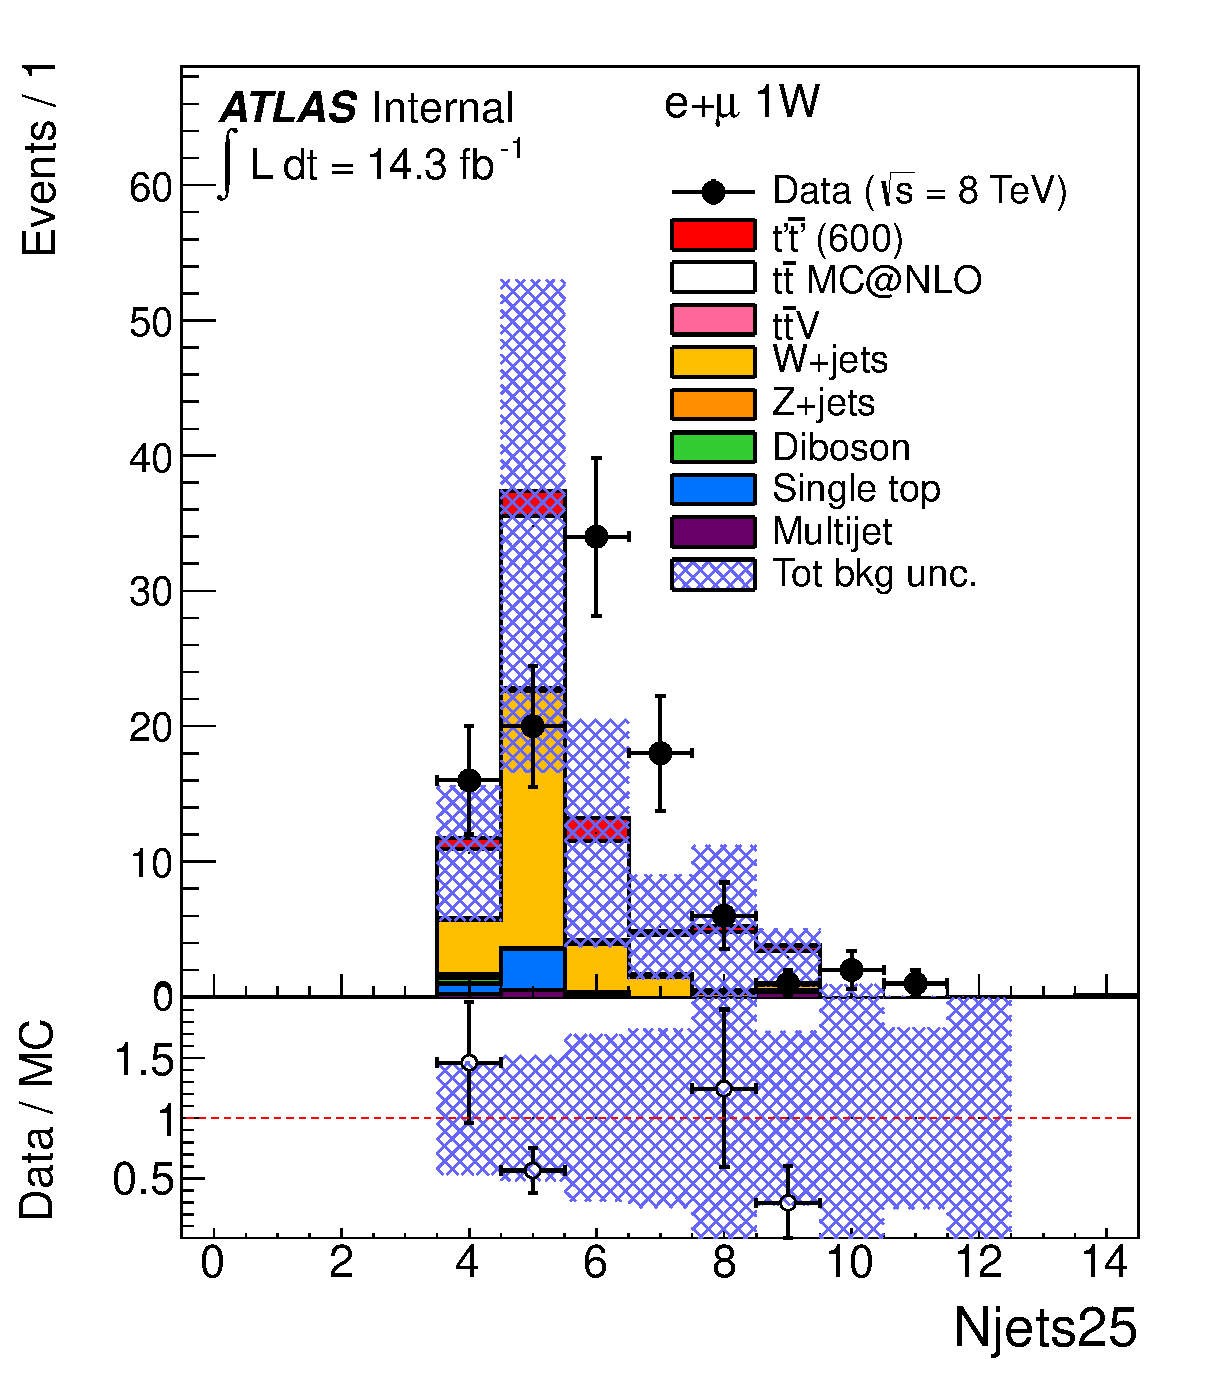
\includegraphics[width=0.30\textwidth]{appendices/figures/sdrs/Njets25_ELEMUONCR8_1W_NOMINAL.eps}  &
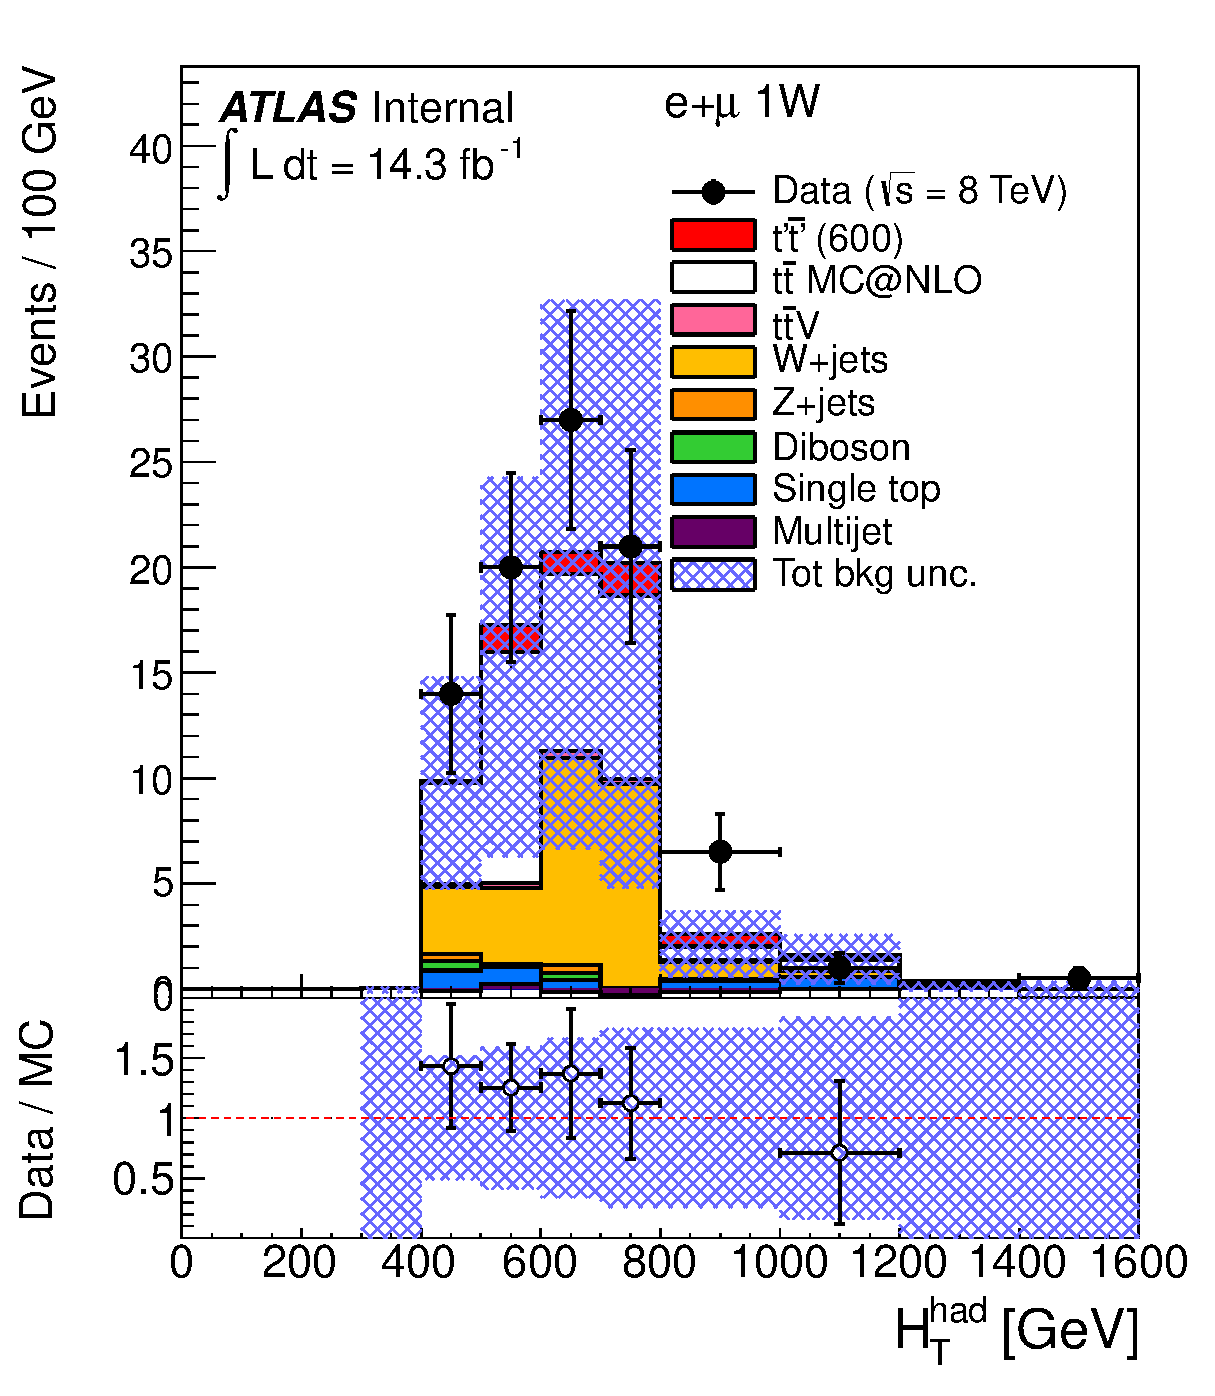
\includegraphics[width=0.30\textwidth]{appendices/figures/sdrs/HTHad_ELEMUONCR8_1W_NOMINAL.eps}  \\
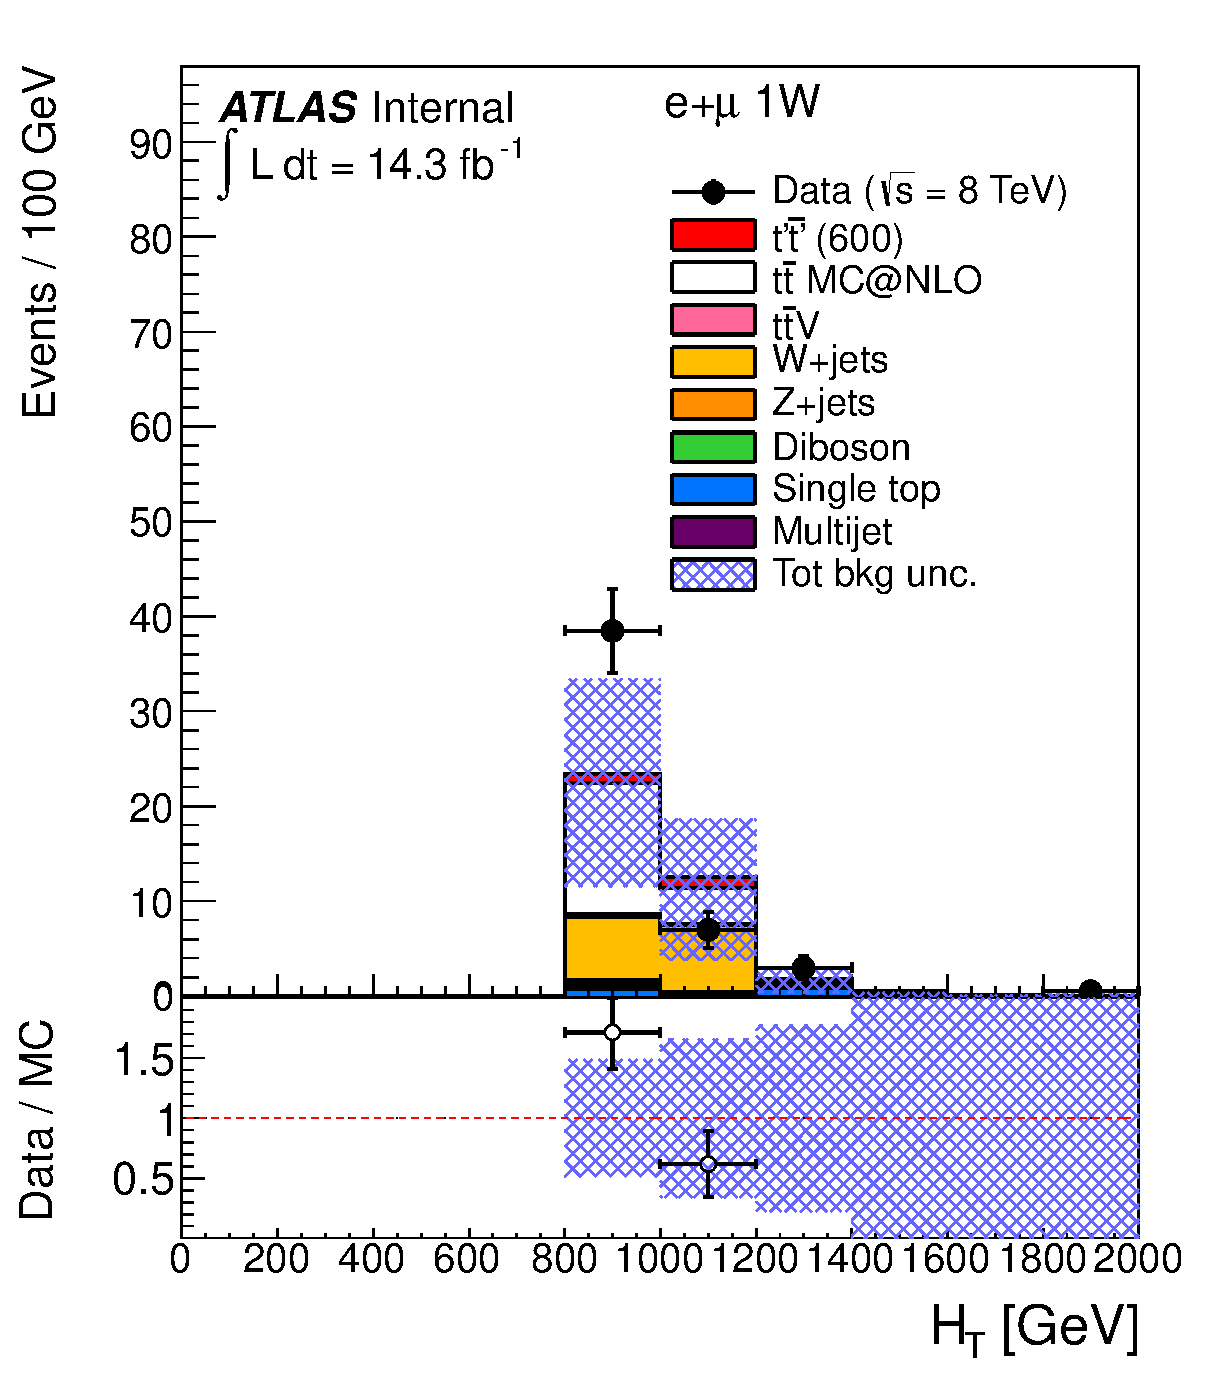
\includegraphics[width=0.30\textwidth]{appendices/figures/sdrs/HTAll_ELEMUONCR8_1W_NOMINAL.eps}  &  &\\
\end{tabular}\caption{\small {Comparison between data and prediction in combined $e$+jets and $\mu$+jets channel in SDR8 (see Sect.~\ref{sec:sdrs} for details) 
for a number of kinematic variables. From top to bottom and left to right, the variables displayed are: lepton $\pt$, lepton $\eta$, missing transverse energy, $W$ transverse mass,
$\hthad$, and $\HT$. The shaded area represents the total background uncertainty.}}
\label{fig:ELEMUONCR8_1}
\end{center}
\end{figure}                                                                             
%%%%%%%%%%%%%%

\clearpage
%%%%%%%%%%%%%%
\begin{figure}[htbp]
\begin{center}
\begin{tabular}{cc}
%
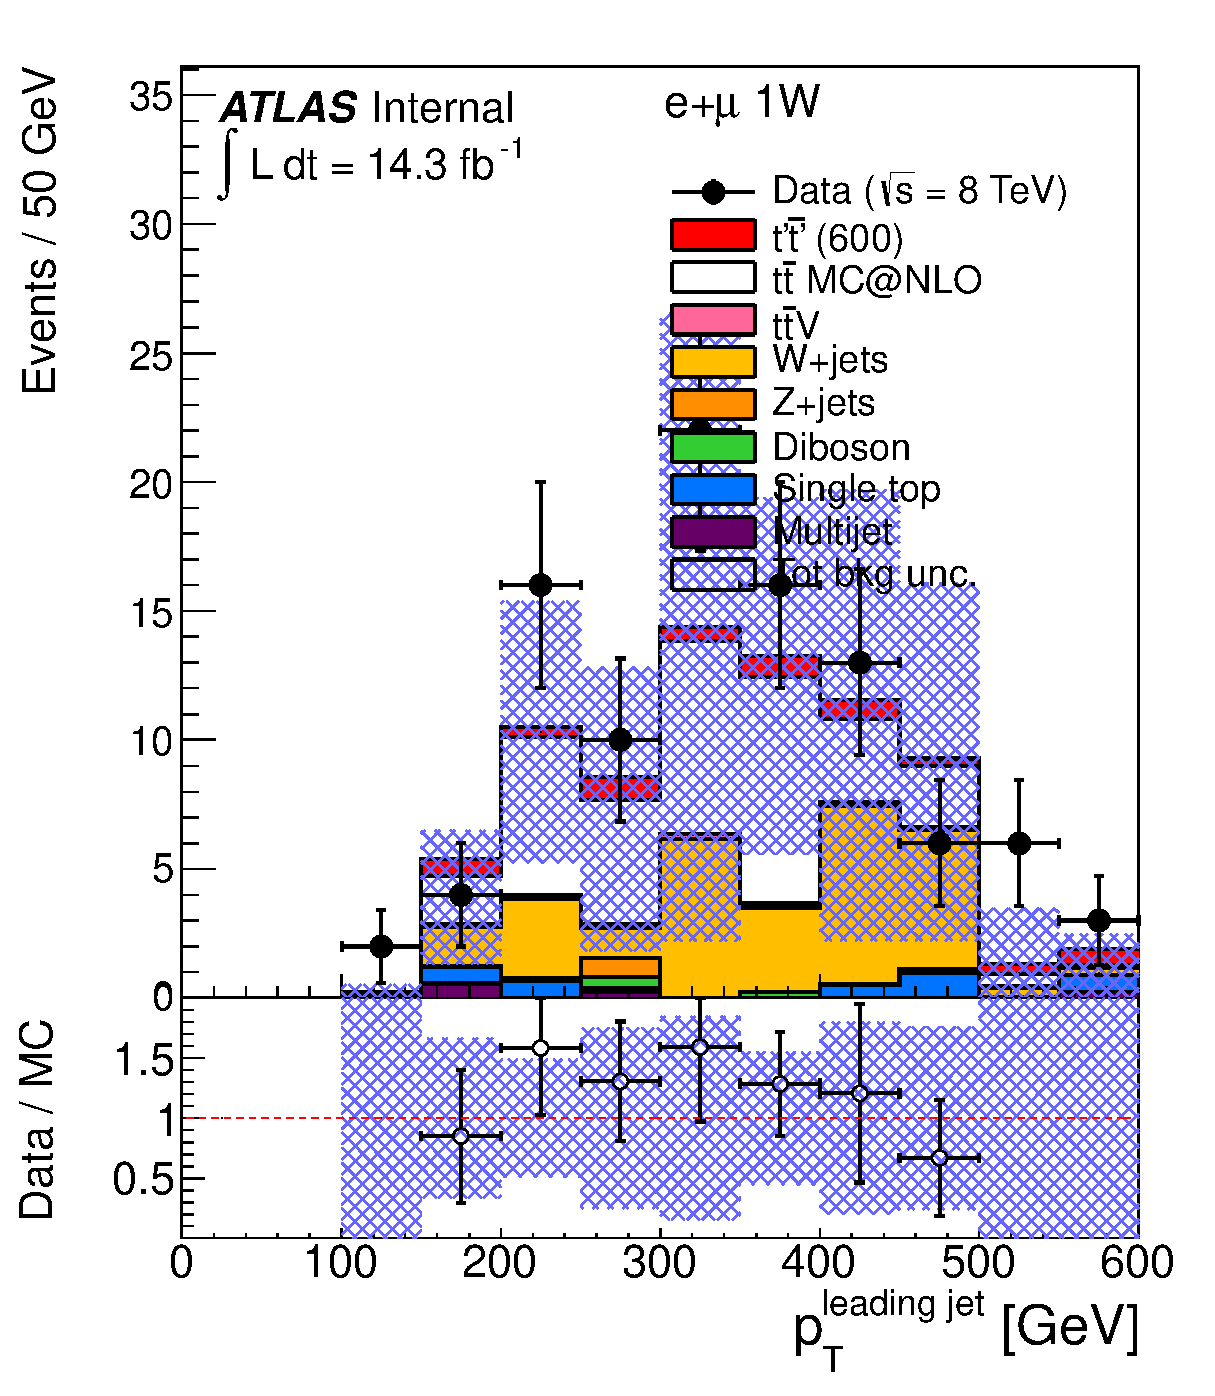
\includegraphics[width=0.30\textwidth]{appendices/figures/sdrs/JetPt1_ELEMUONCR8_1W_NOMINAL.eps} &
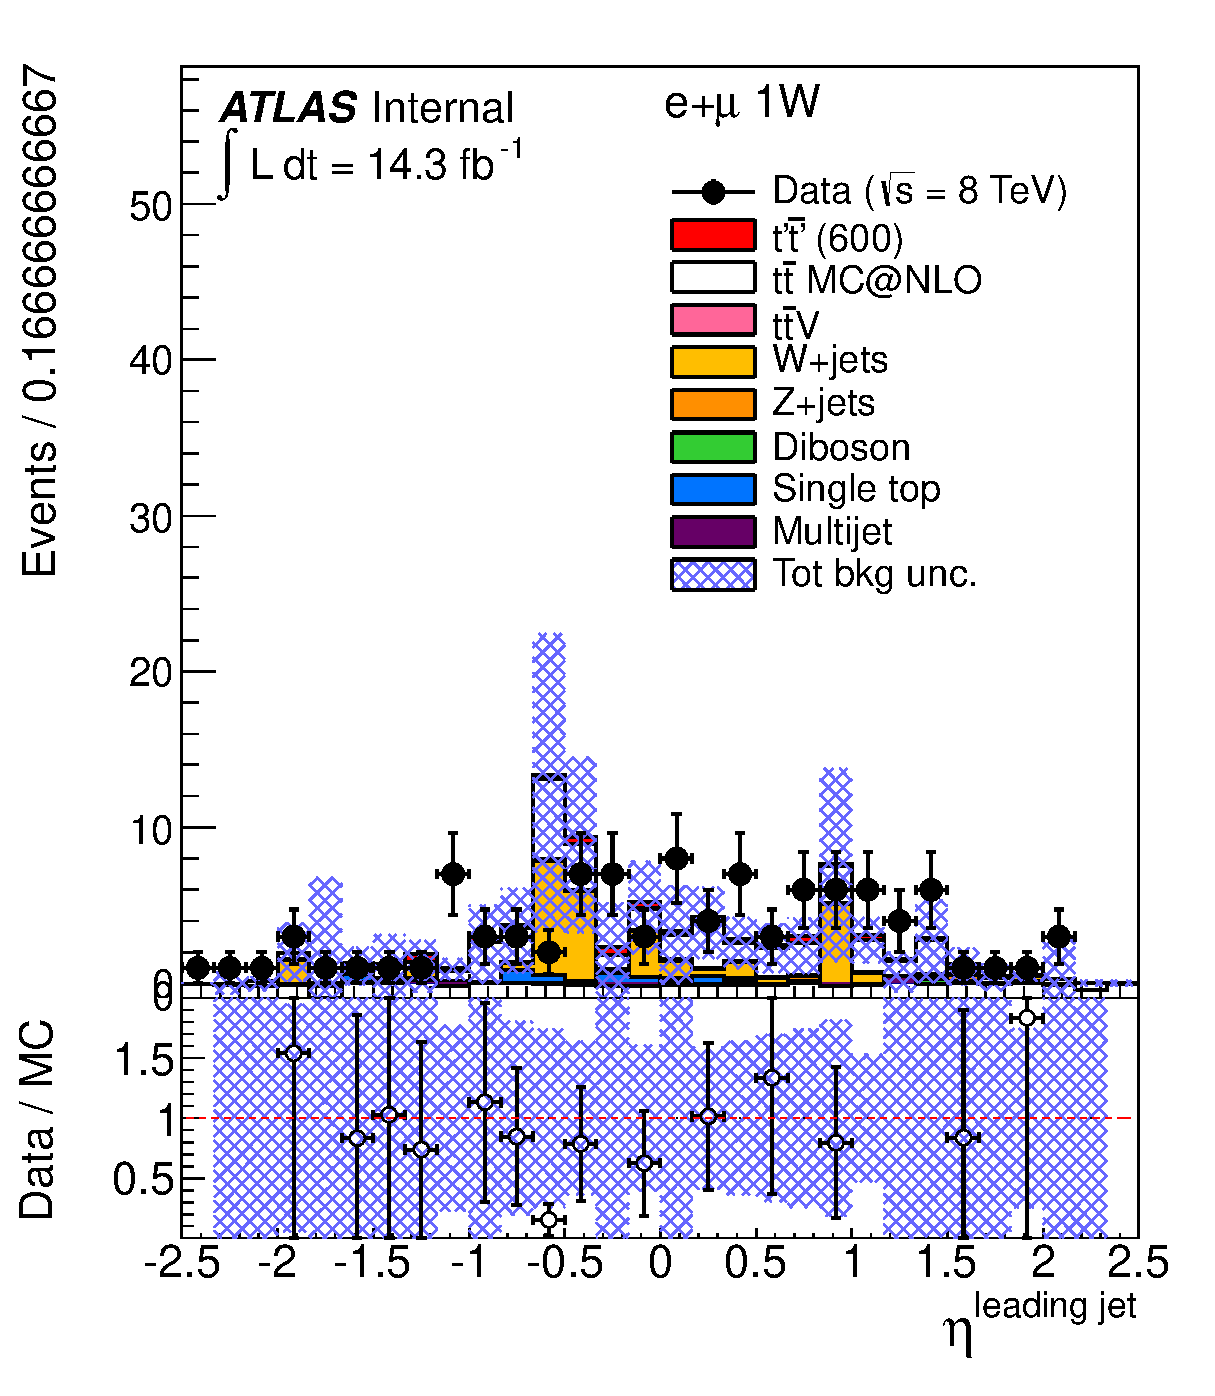
\includegraphics[width=0.30\textwidth]{appendices/figures/sdrs/JetEta1_ELEMUONCR8_1W_NOMINAL.eps} \\
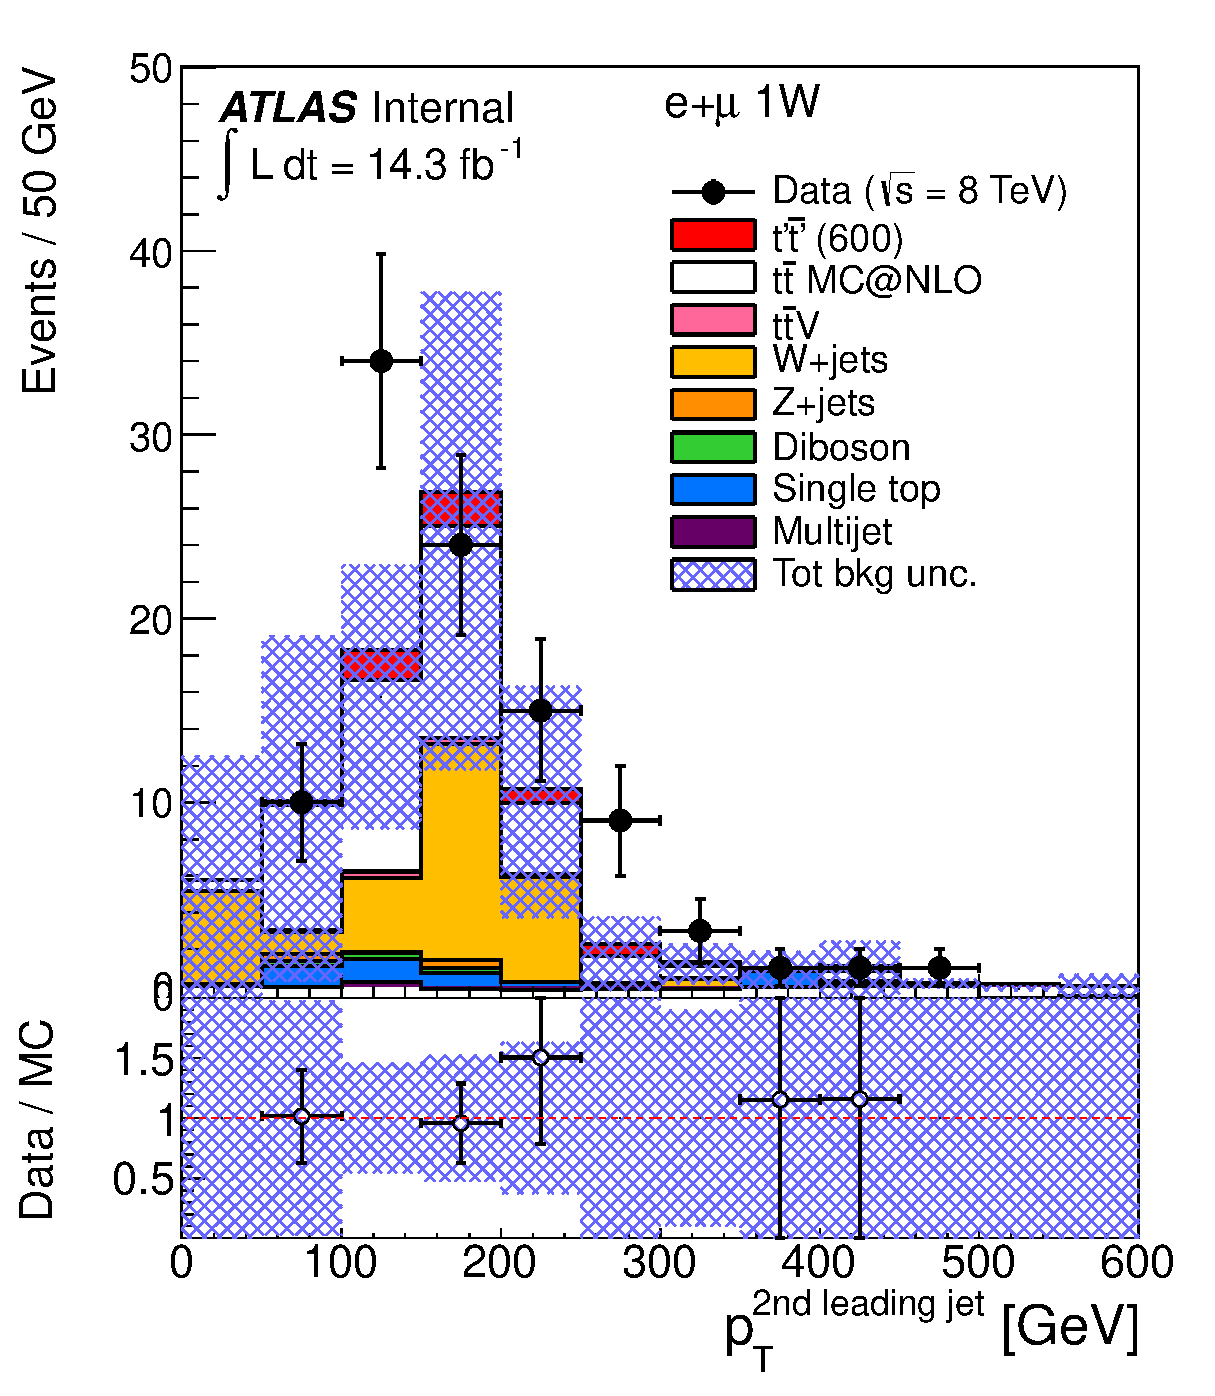
\includegraphics[width=0.30\textwidth]{appendices/figures/sdrs/JetPt2_ELEMUONCR8_1W_NOMINAL.eps} &
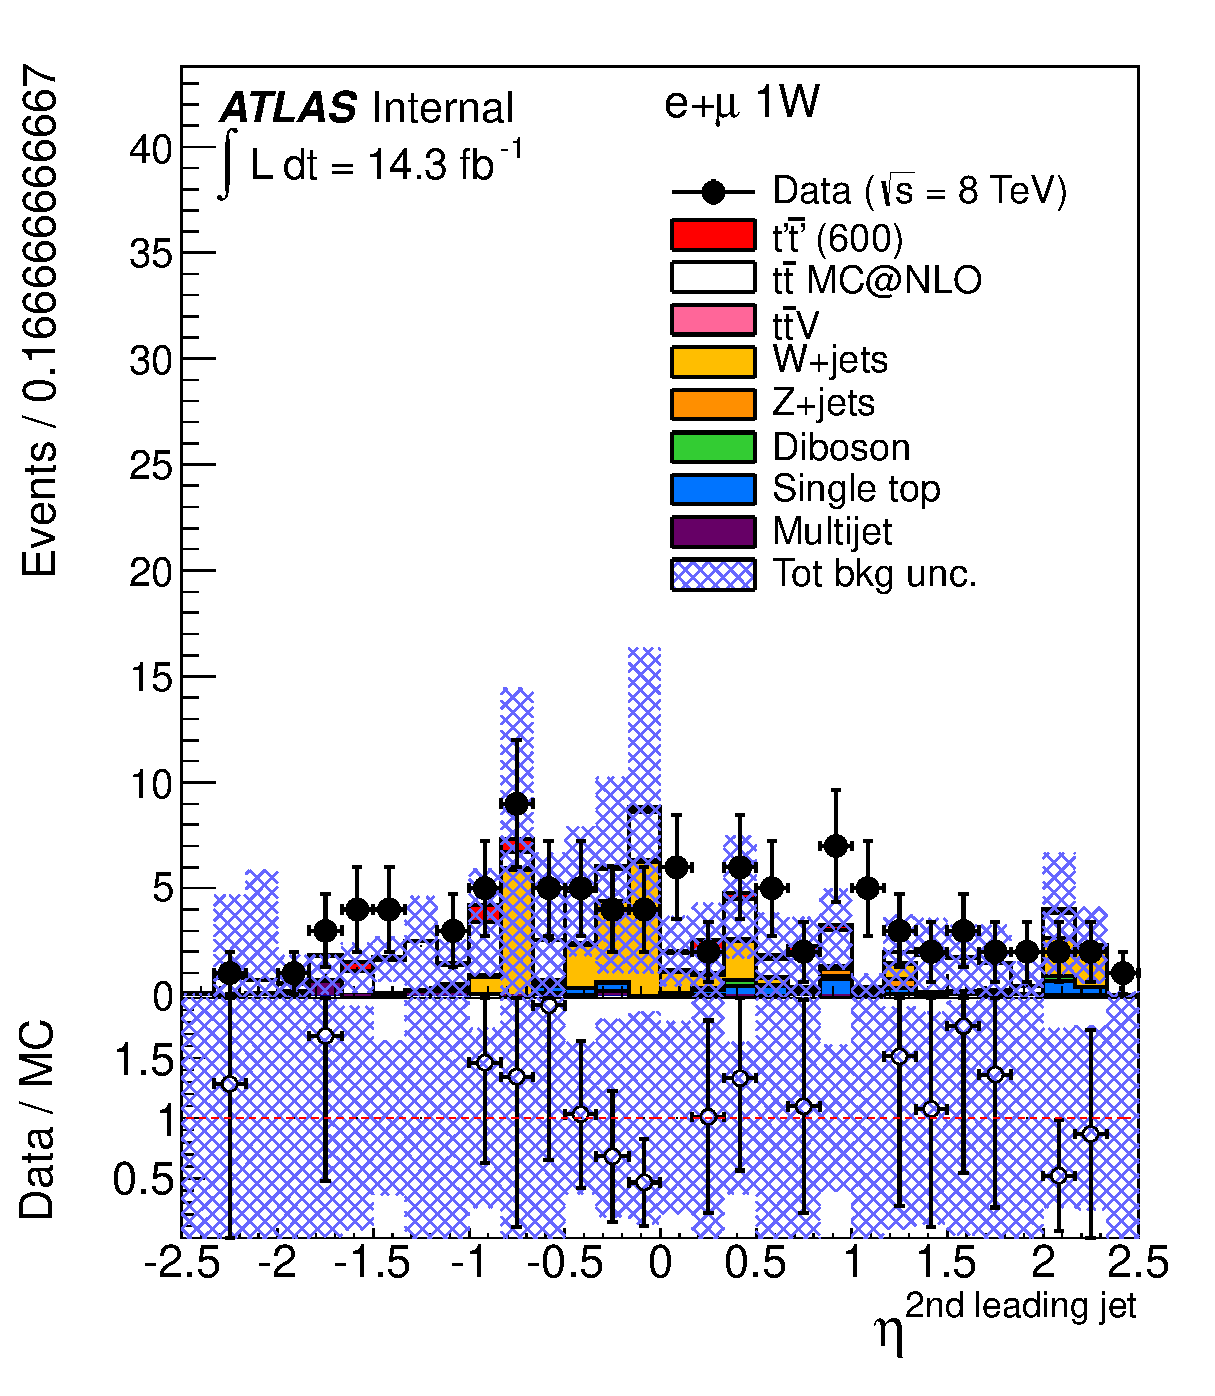
\includegraphics[width=0.30\textwidth]{appendices/figures/sdrs/JetEta2_ELEMUONCR8_1W_NOMINAL.eps} \\
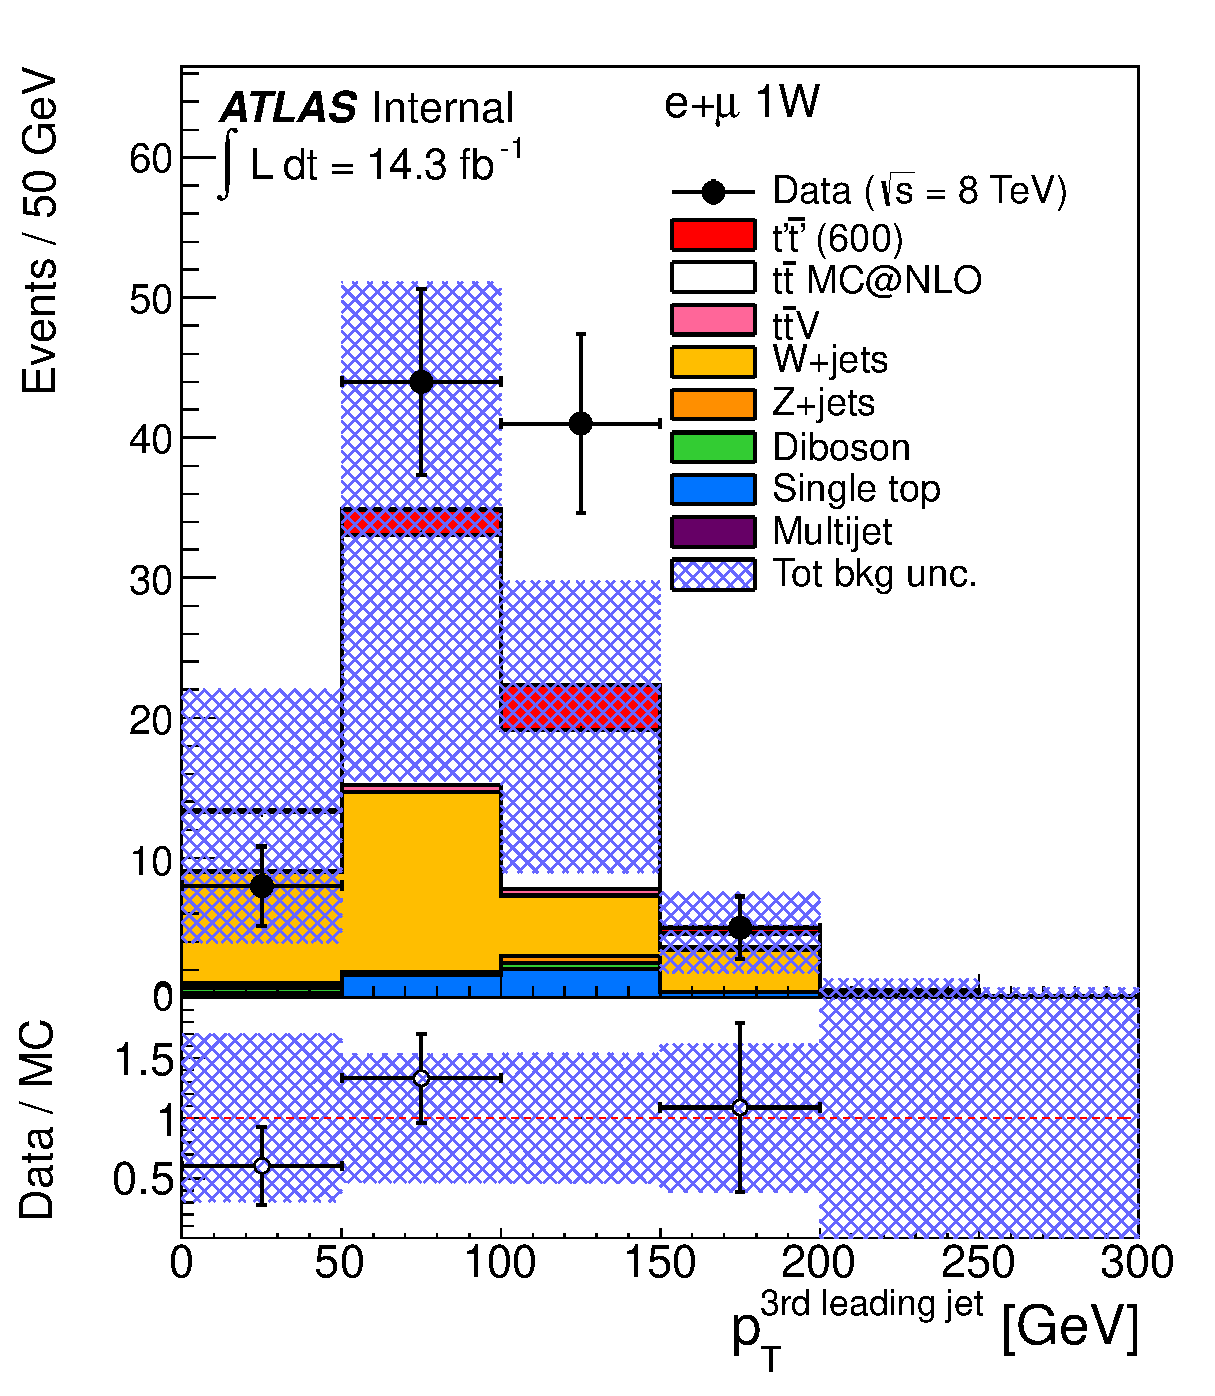
\includegraphics[width=0.30\textwidth]{appendices/figures/sdrs/JetPt3_ELEMUONCR8_1W_NOMINAL.eps} &
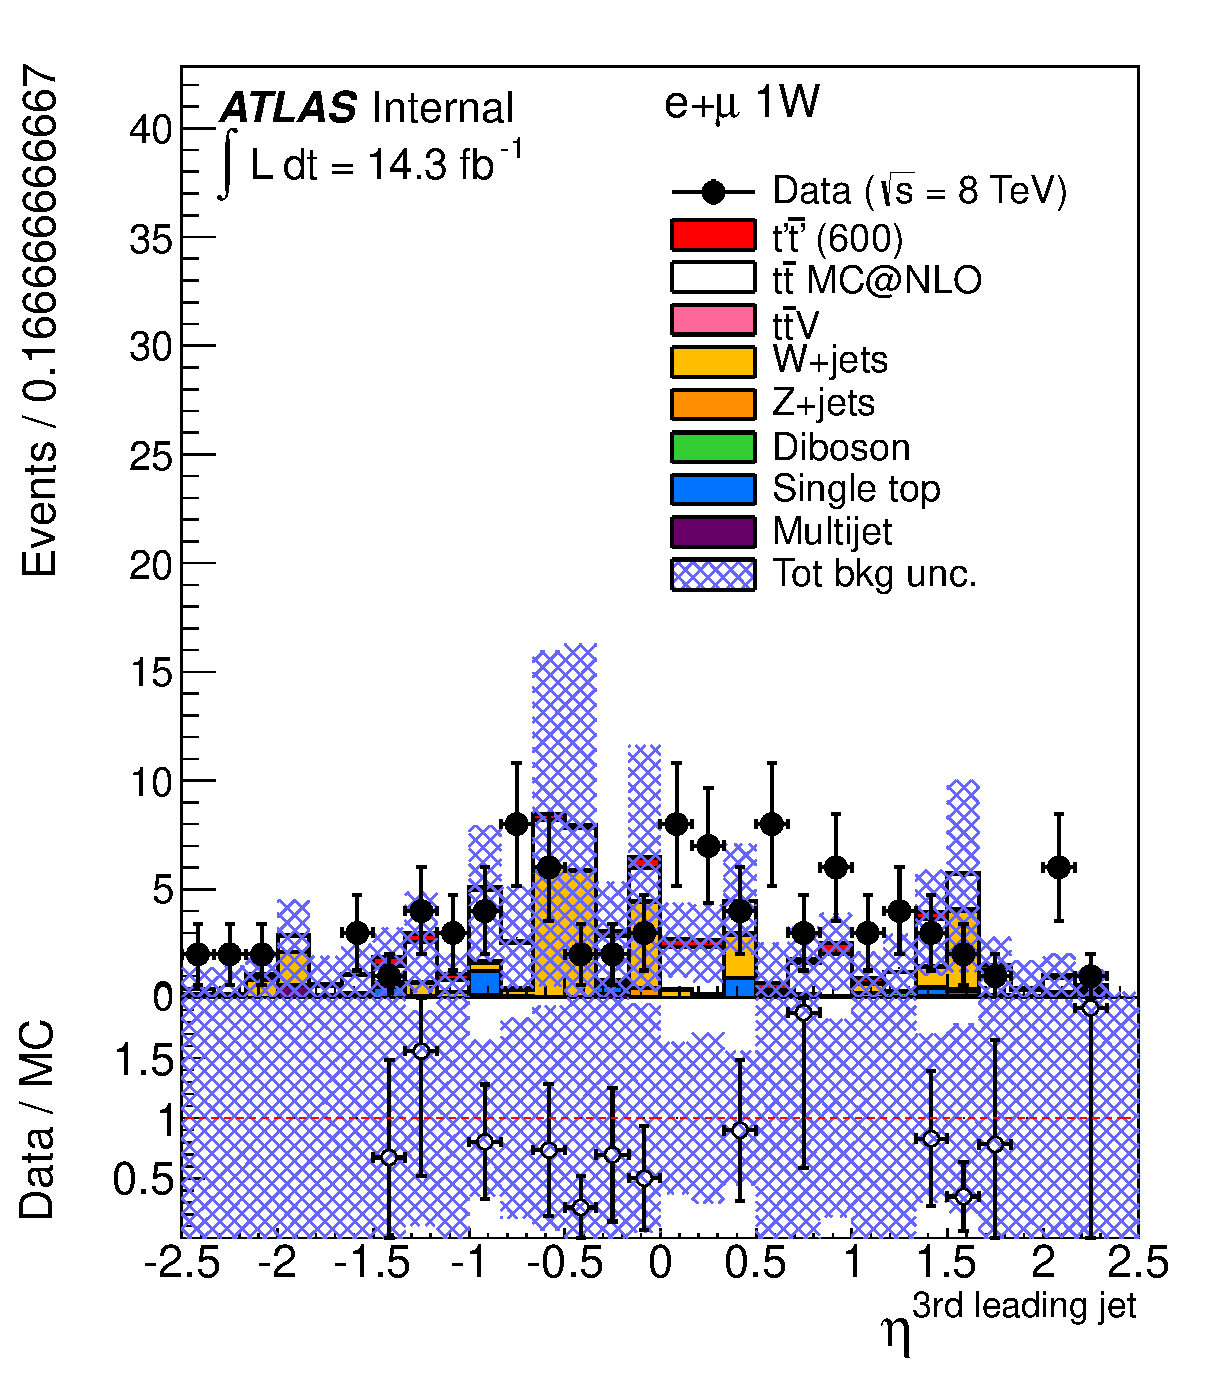
\includegraphics[width=0.30\textwidth]{appendices/figures/sdrs/JetEta3_ELEMUONCR8_1W_NOMINAL.eps} \\
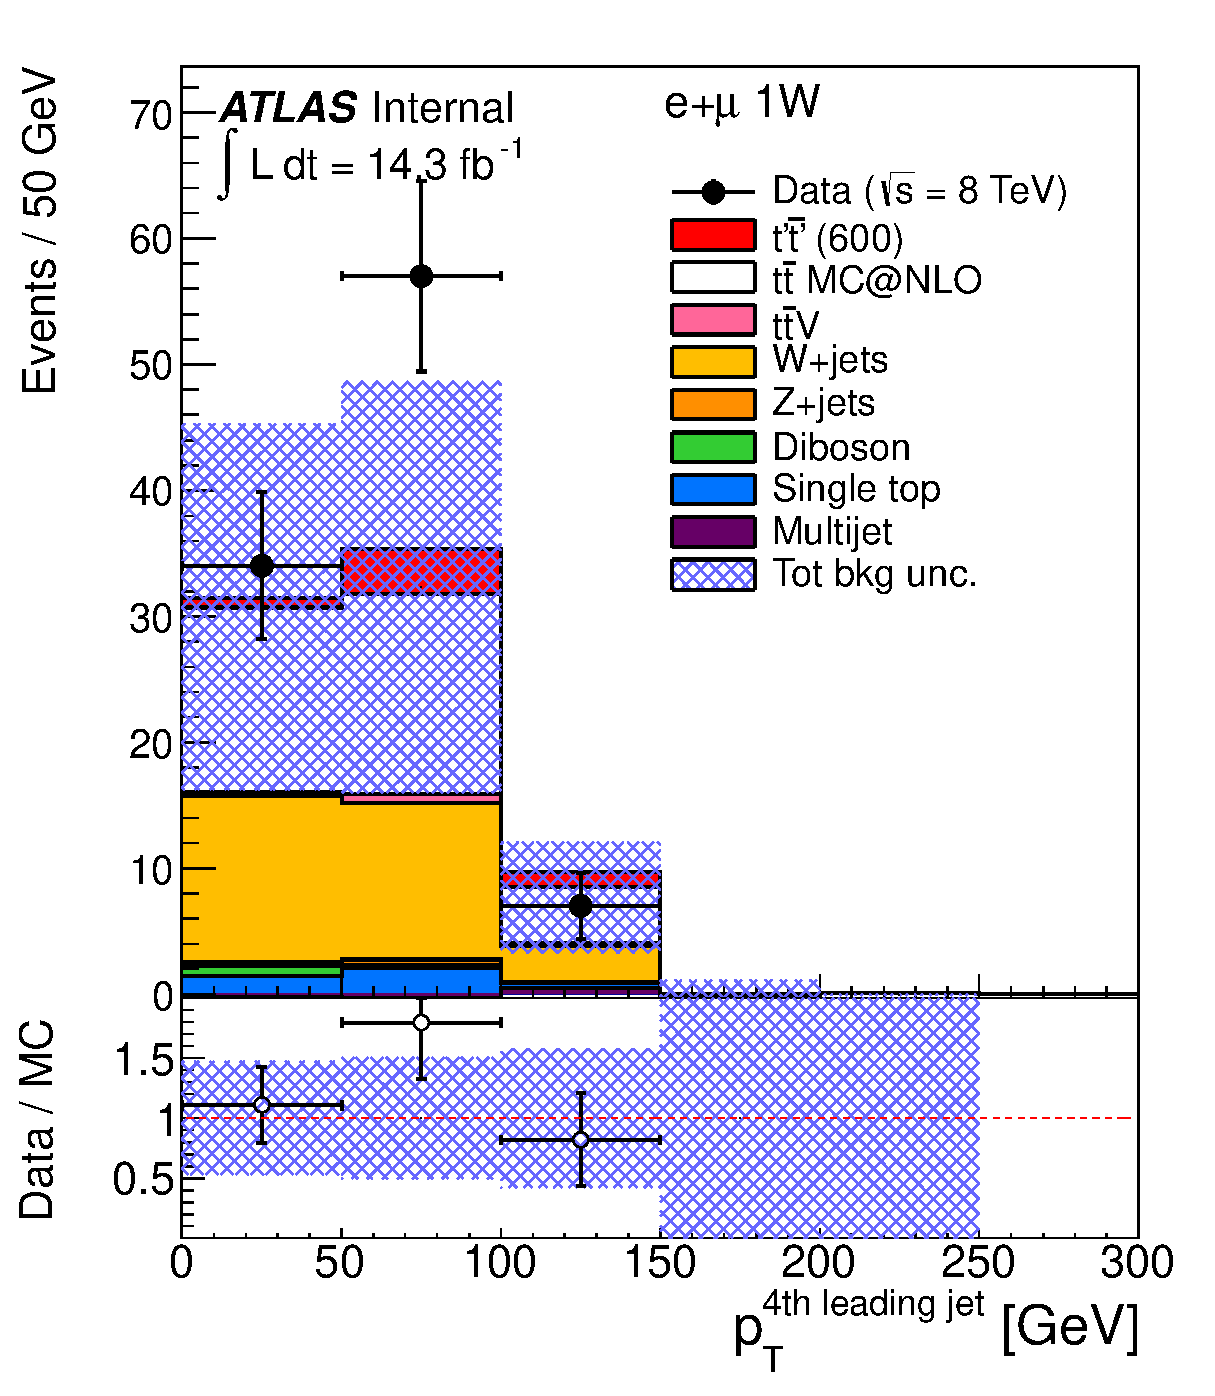
\includegraphics[width=0.30\textwidth]{appendices/figures/sdrs/JetPt4_ELEMUONCR8_1W_NOMINAL.eps}  &
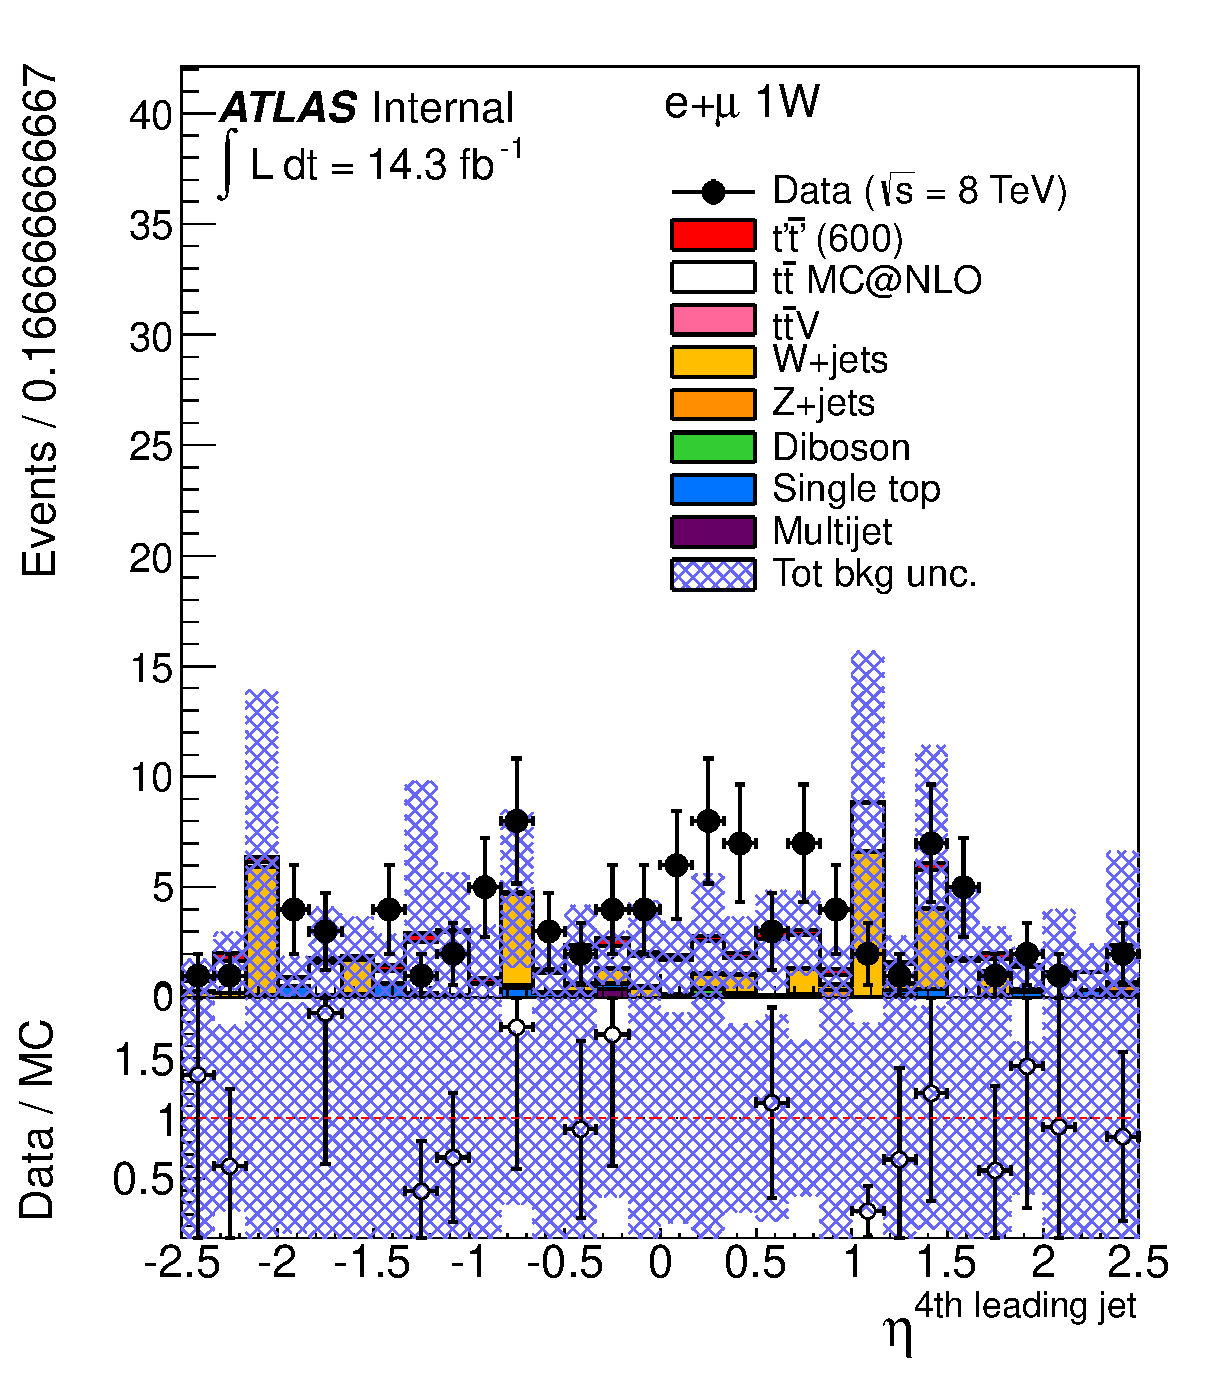
\includegraphics[width=0.30\textwidth]{appendices/figures/sdrs/JetEta4_ELEMUONCR8_1W_NOMINAL.eps}  \\
\end{tabular}\caption{\small {Comparison between data and prediction in combined $e$+jets and $\mu$+jets channel in SDR8 (see Sect.~\ref{sec:sdrs} for details) 
for a number of kinematic variables. From top to bottom and left to right, the variables displayed are: leading jet $\pt$ and $\eta$,  second leading jet $\pt$ and $\eta$,
third leading jet $\pt$ and $\eta$, and fourth leading jet $\pt$ and $\eta$. The shaded area represents the total background uncertainty.}}
\label{fig:ELEMUONCR8_2}
\end{center}
\end{figure}                                                                             
%%%%%%%%%%%%%%

\clearpage
%%%%%%%%%%%%%%
\begin{figure}[htbp]
\begin{center}
\begin{tabular}{ccc}
%
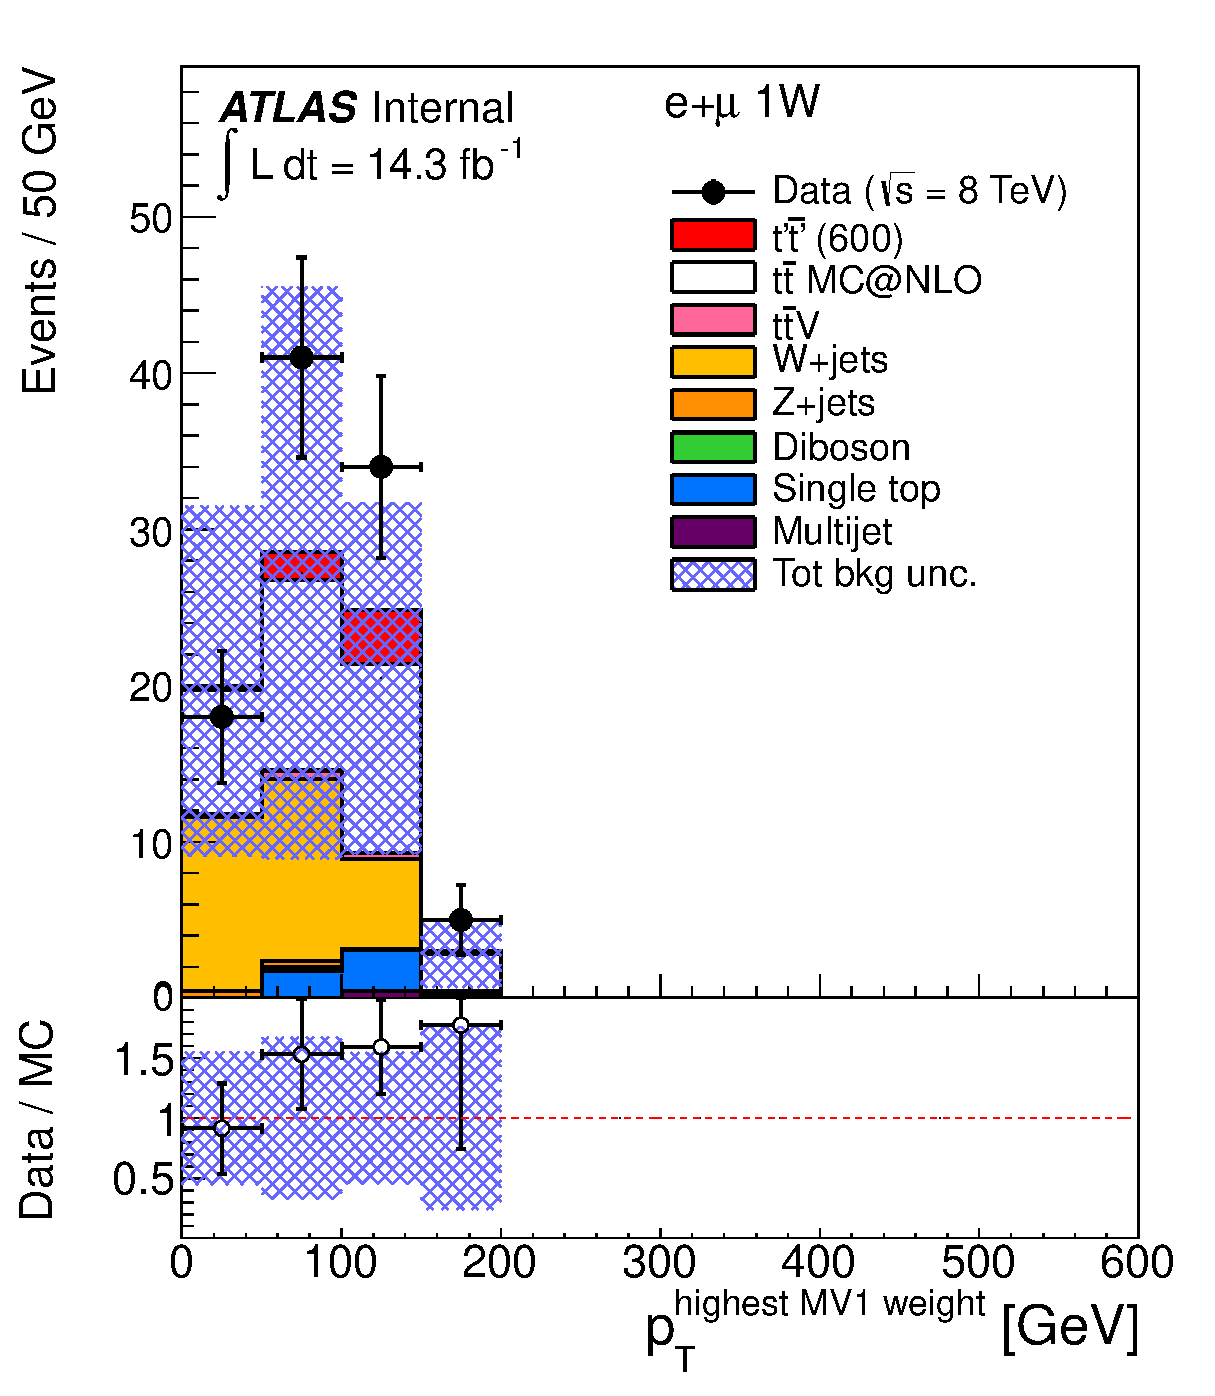
\includegraphics[width=0.30\textwidth]{appendices/figures/sdrs/JetPtB1_ELEMUONCR8_1W_NOMINAL.eps}  &
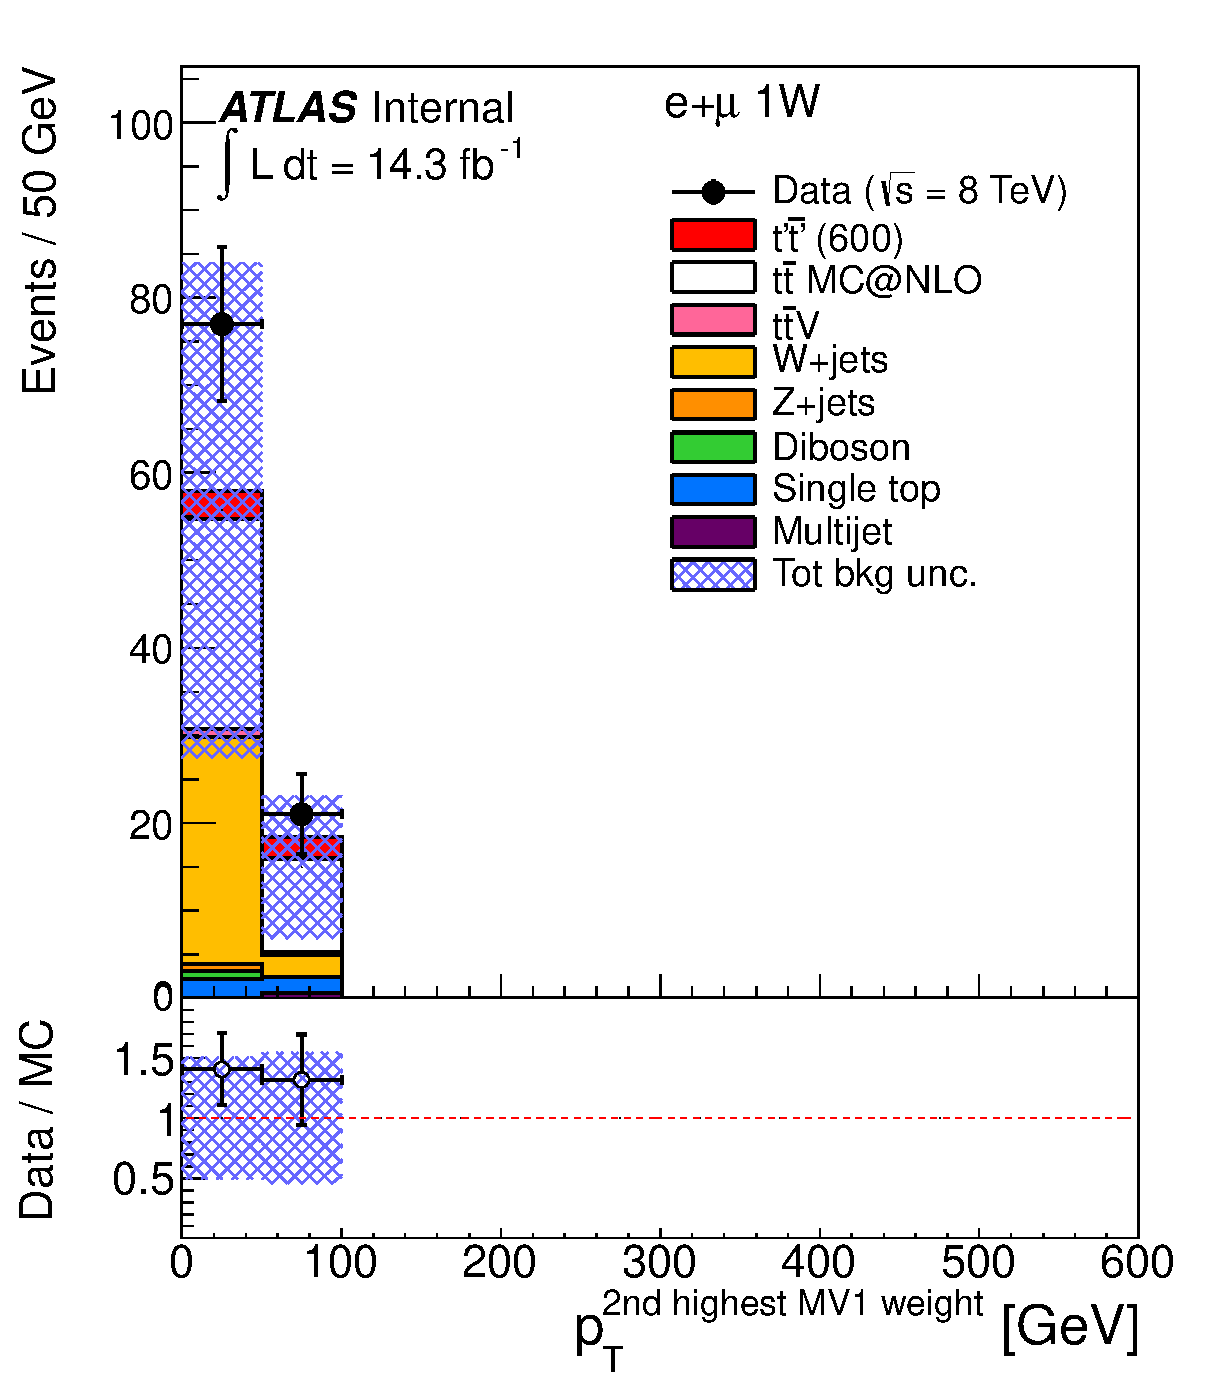
\includegraphics[width=0.30\textwidth]{appendices/figures/sdrs/JetPtB2_ELEMUONCR8_1W_NOMINAL.eps} &
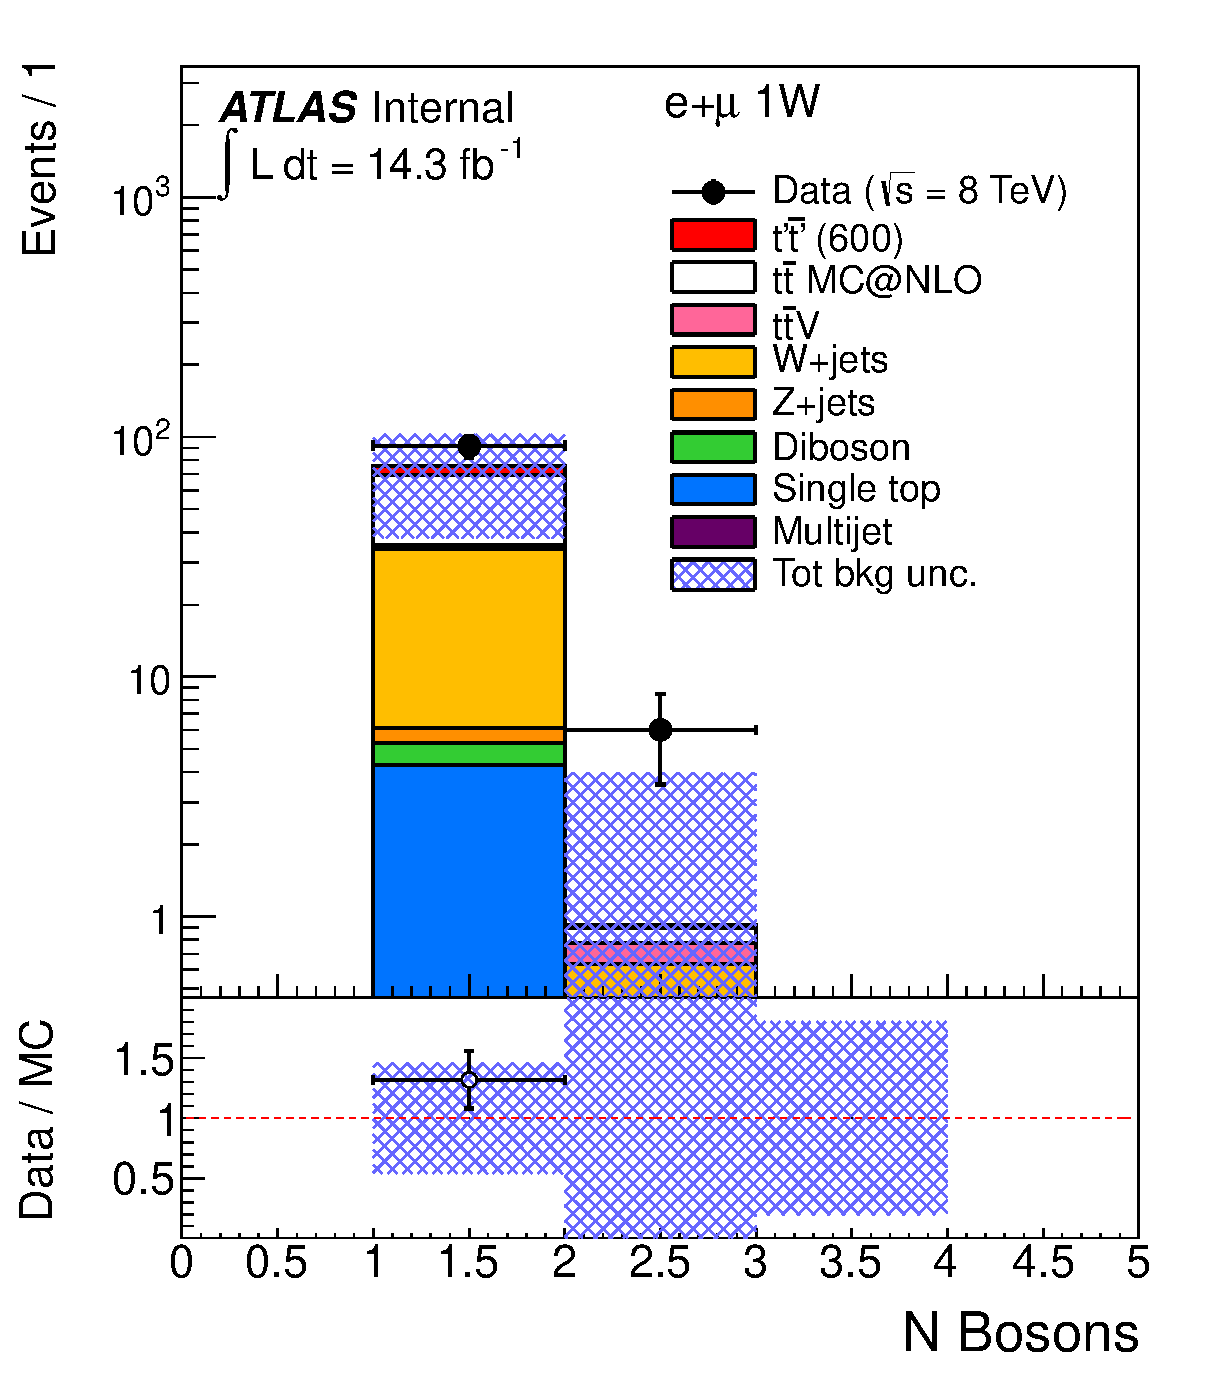
\includegraphics[width=0.30\textwidth]{appendices/figures/sdrs/nWhad_ELEMUONCR8_1W_NOMINAL_logscale.eps} \\
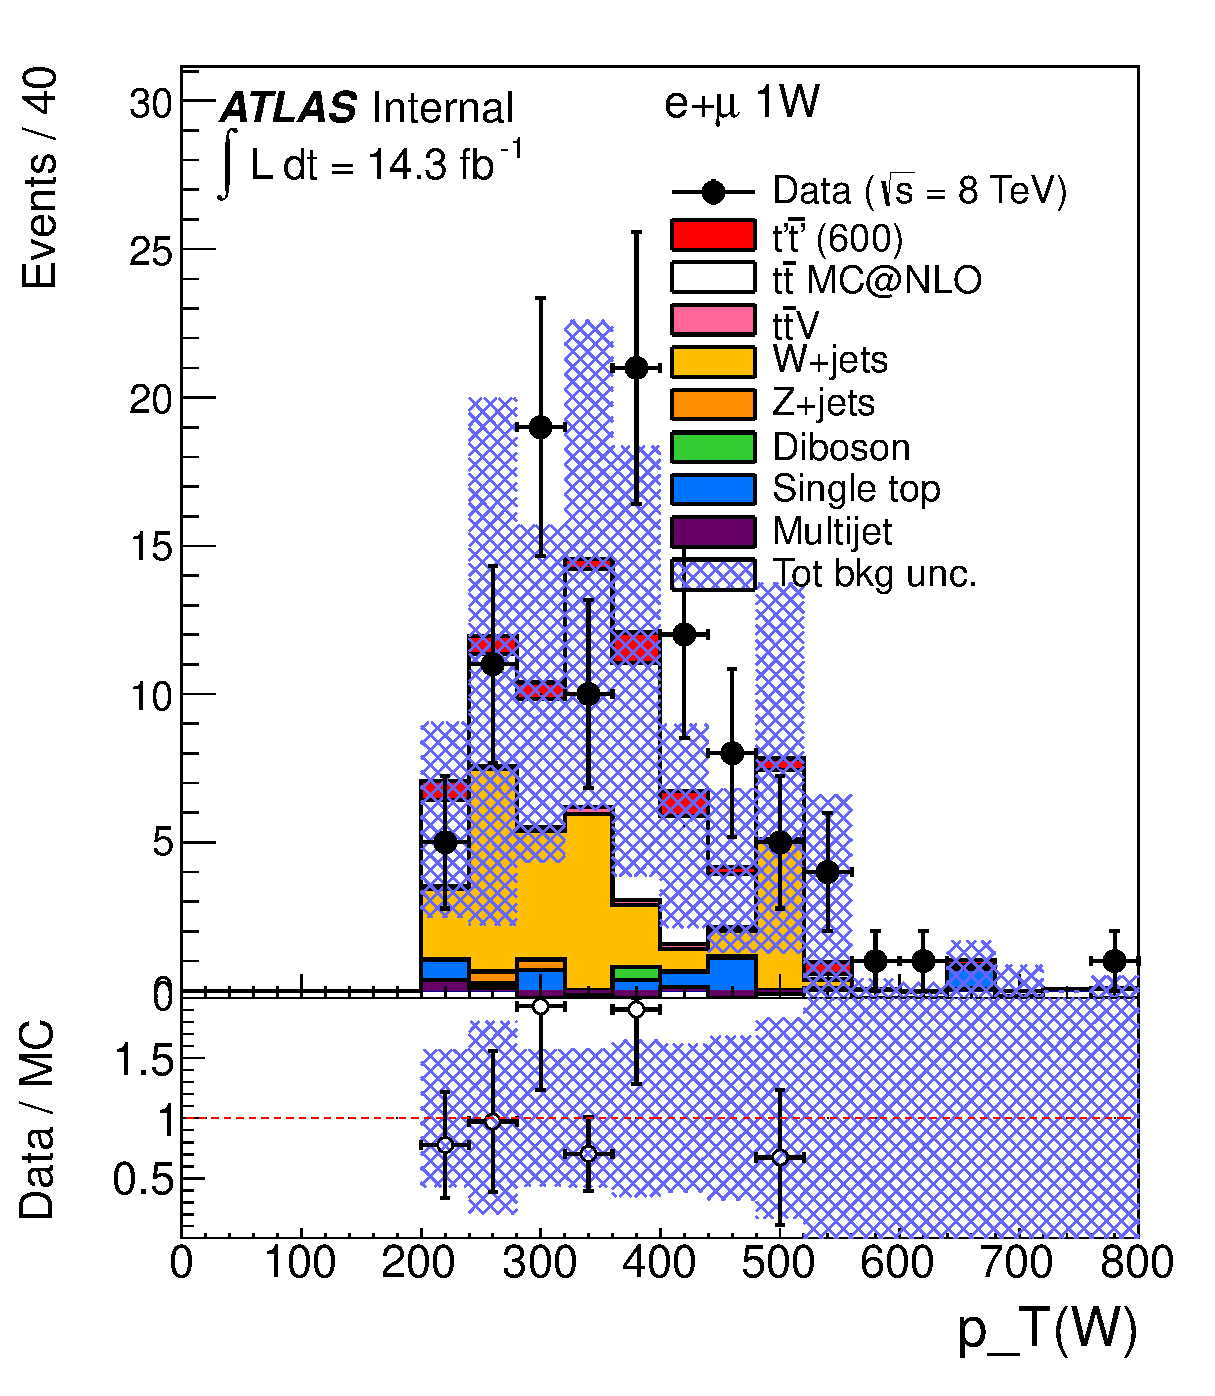
\includegraphics[width=0.30\textwidth]{appendices/figures/sdrs/VLQAna_WbX_W1Pt_ELEMUONCR8_1W_NOMINAL.eps} &
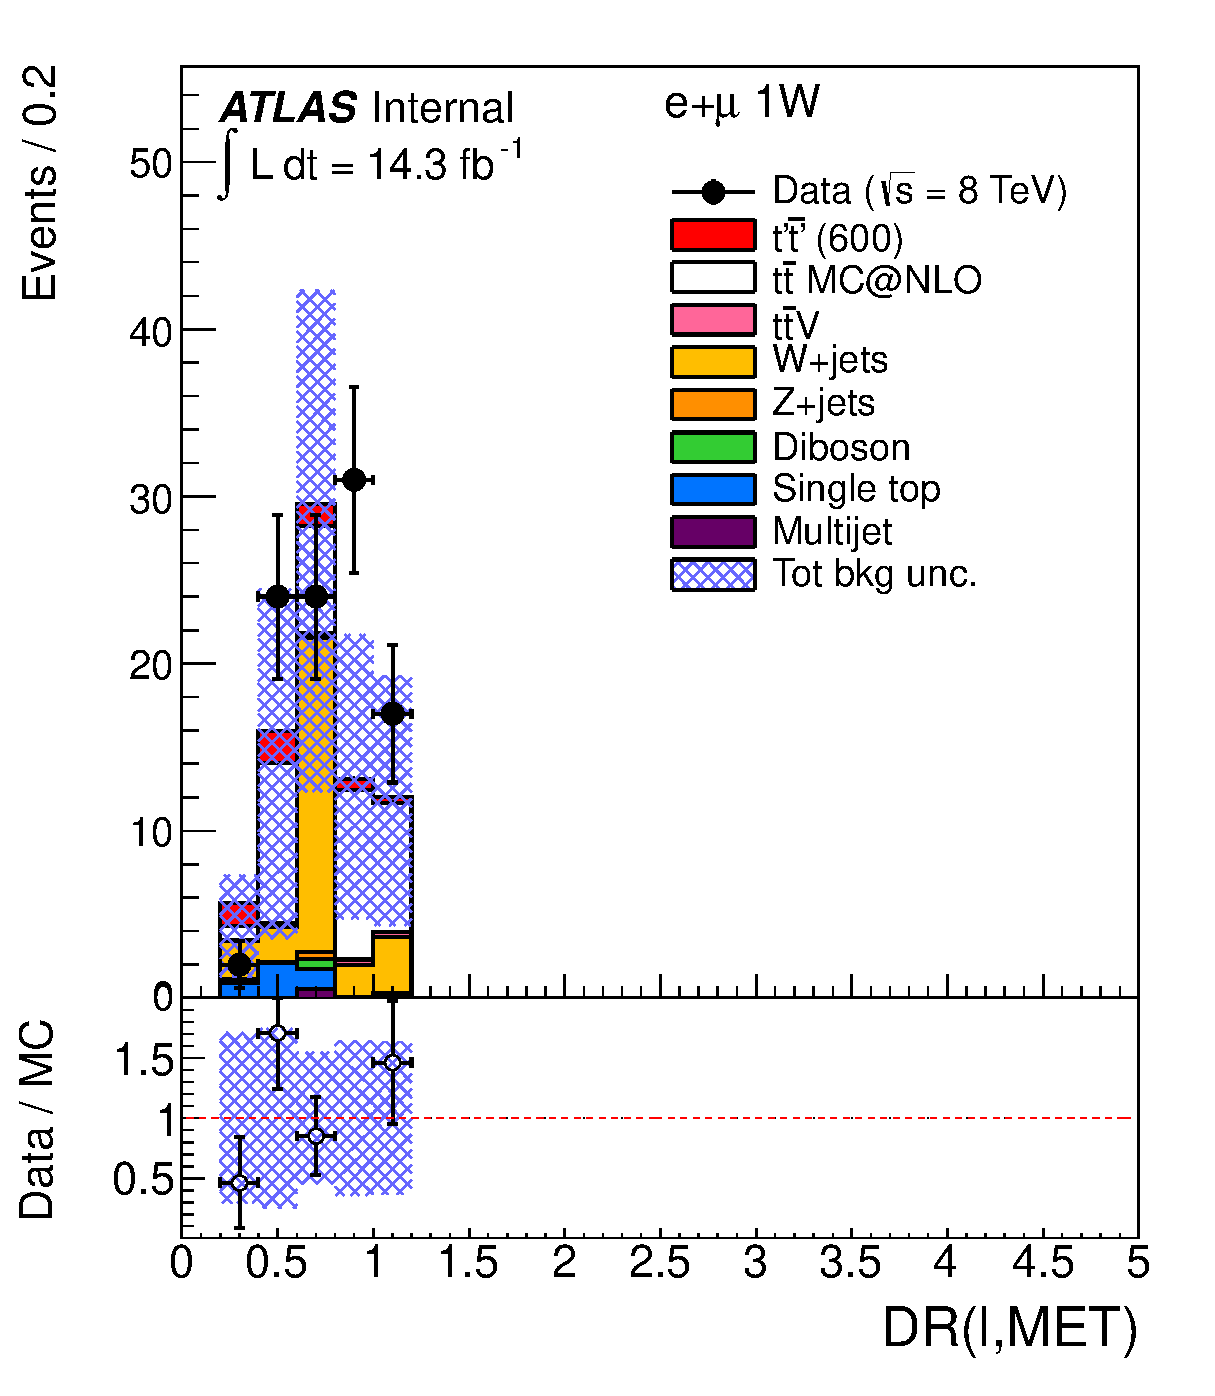
\includegraphics[width=0.30\textwidth]{appendices/figures/sdrs/VLQAna_WbX_DRLepMet_ELEMUONCR8_1W_NOMINAL.eps} &
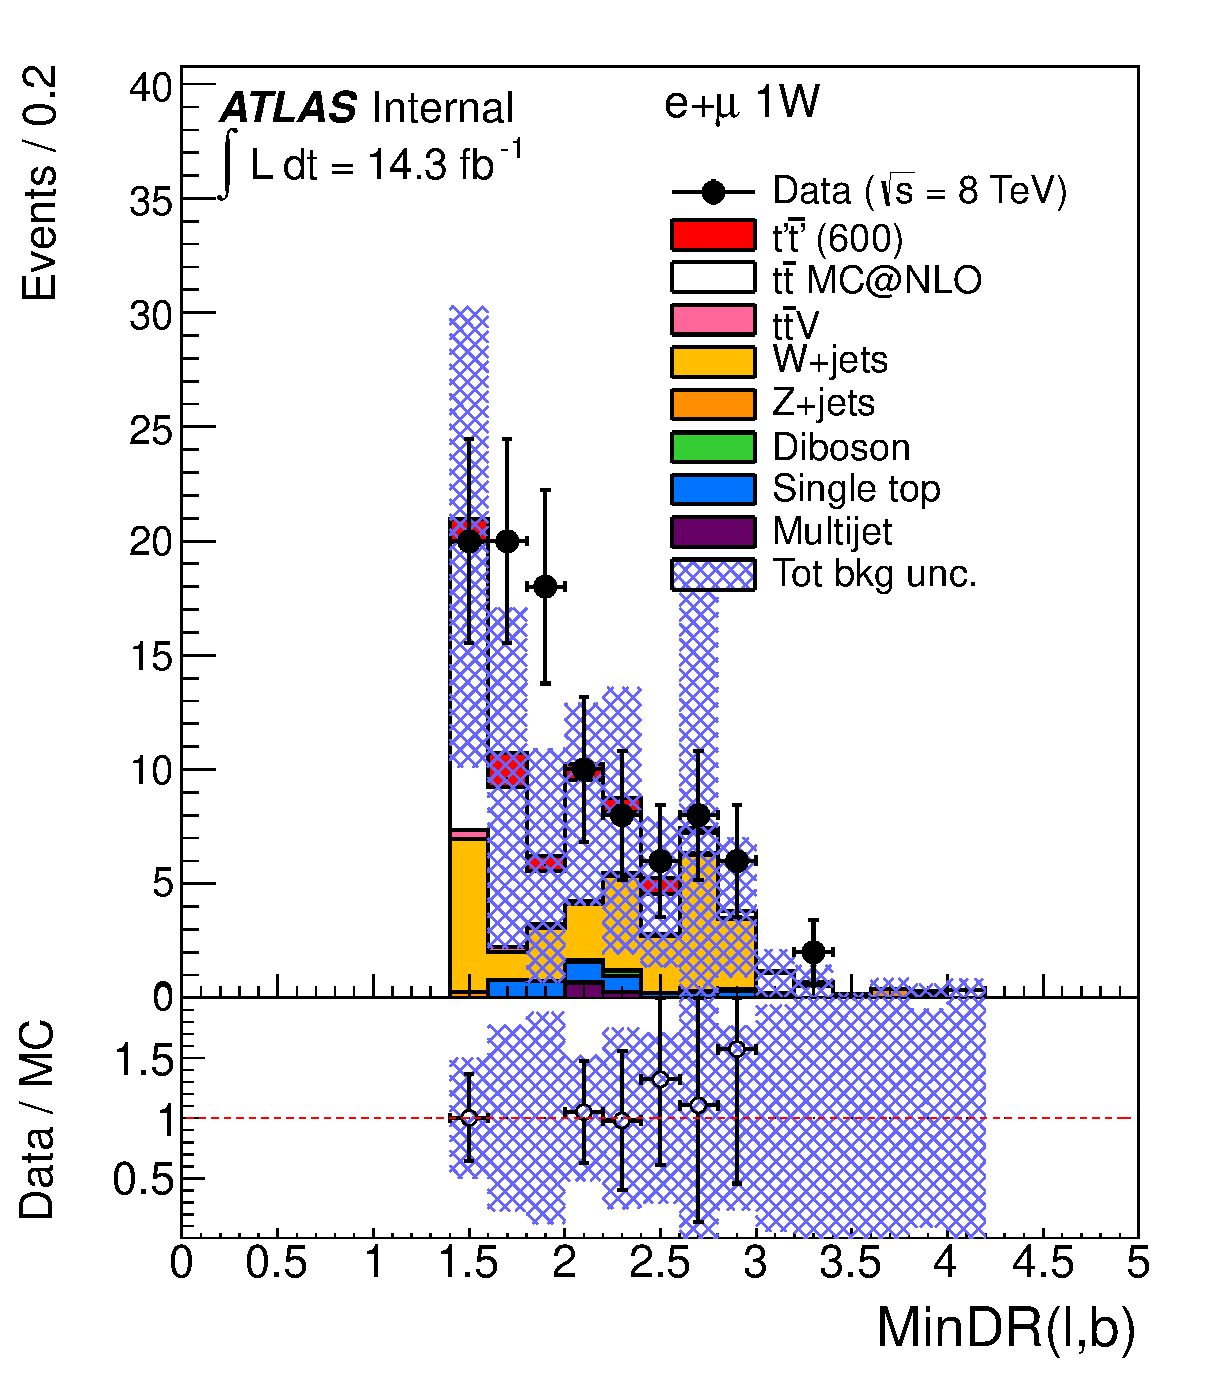
\includegraphics[width=0.30\textwidth]{appendices/figures/sdrs/VLQAna_WbX_MinDRlb_ELEMUONCR8_1W_NOMINAL.eps} \\
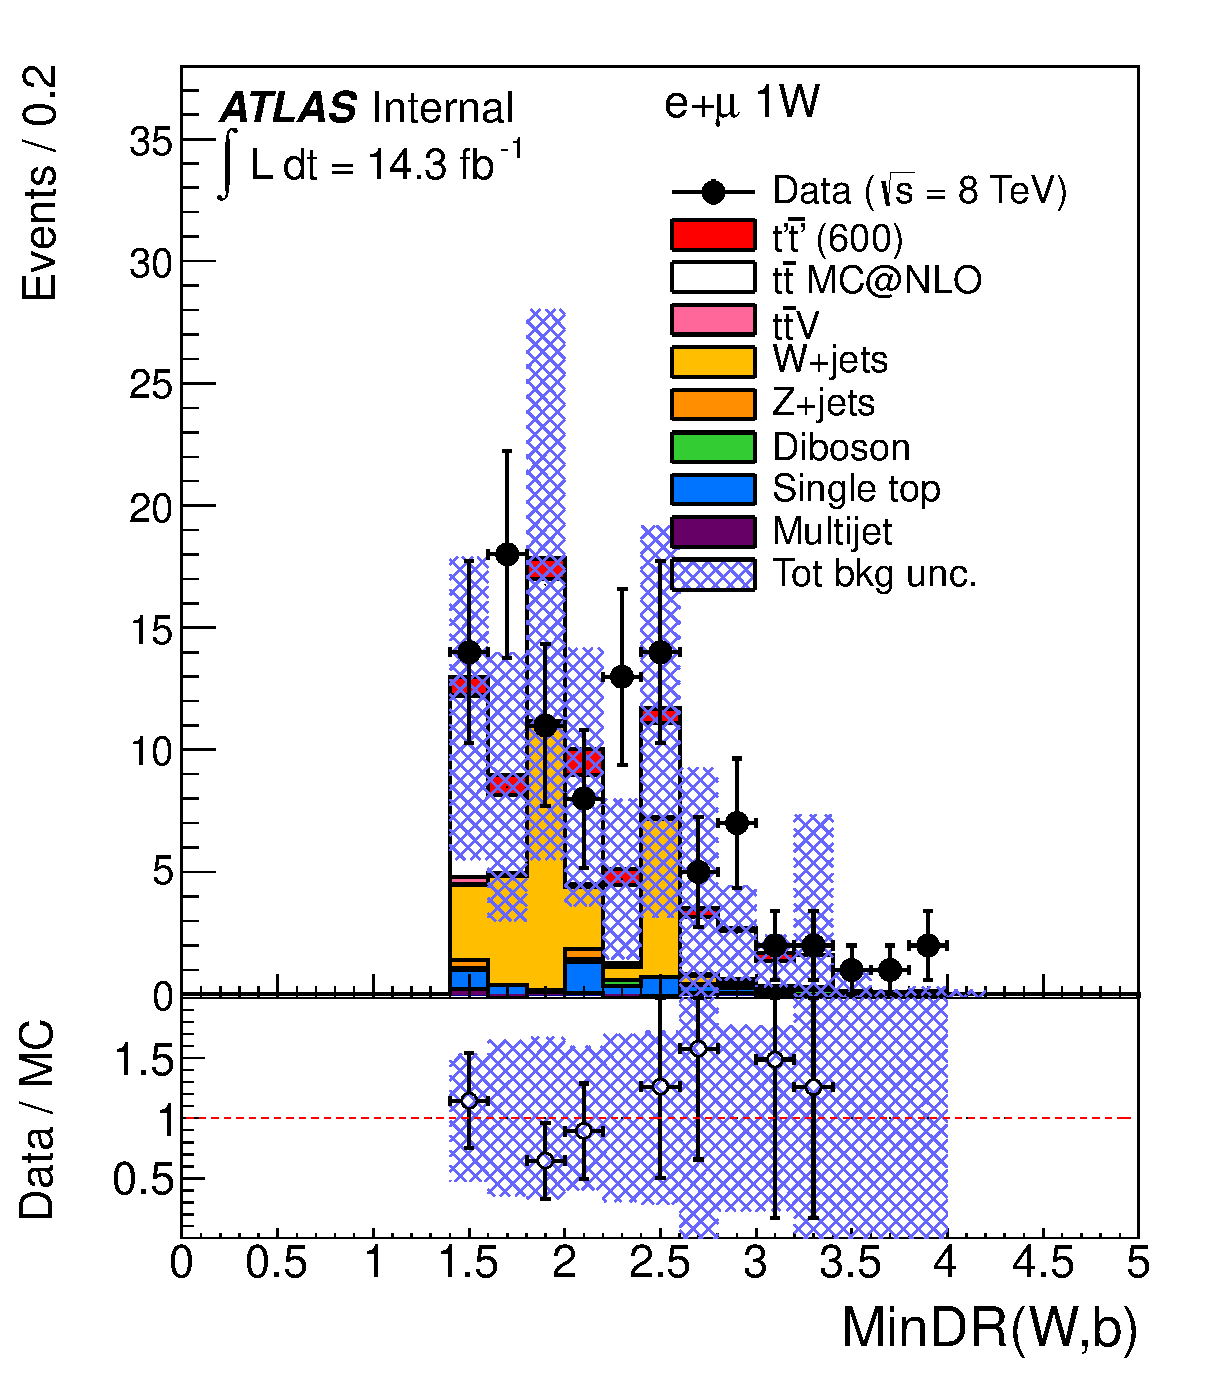
\includegraphics[width=0.30\textwidth]{appendices/figures/sdrs/VLQAna_WbX_MinDRWb_ELEMUONCR8_1W_NOMINAL.eps} &
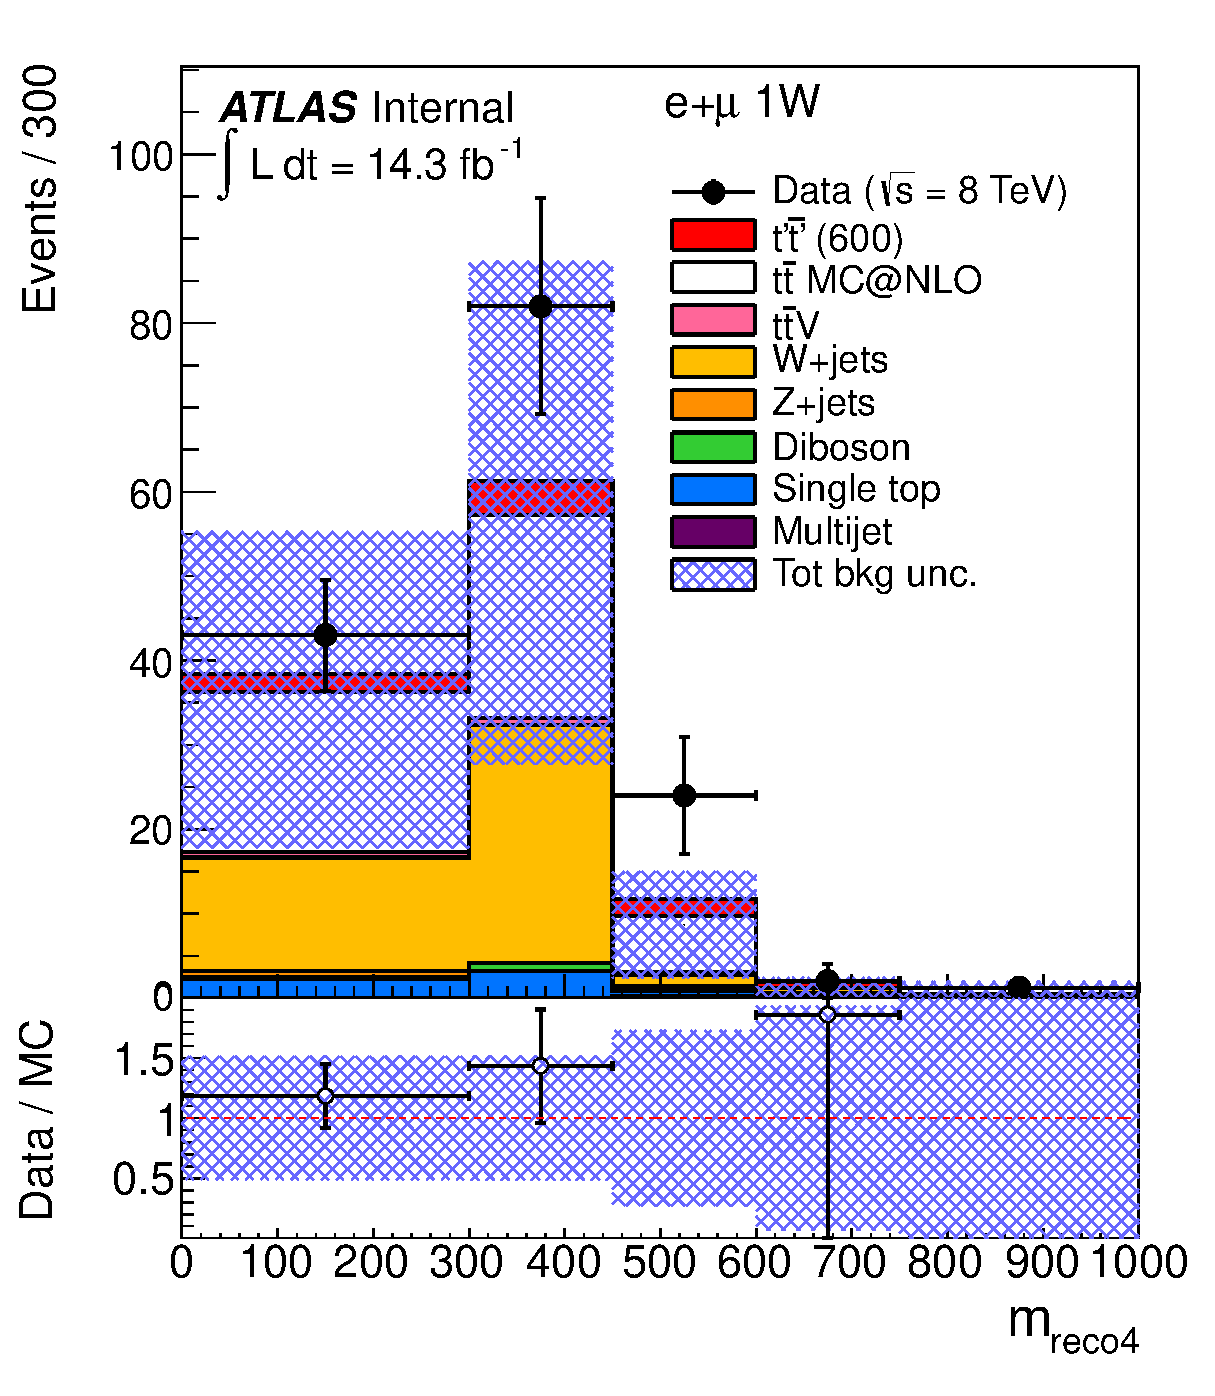
\includegraphics[width=0.30\textwidth]{appendices/figures/sdrs/VLQAna_WbX_1W_MWb_4_ELEMUONCR8_1W_NOMINAL.eps} & \\
\end{tabular}\caption{\small {Comparison between data and prediction in combined $e$+jets and $\mu$+jets channel in SDR8 (see Sect.~\ref{sec:sdrs} for details) 
for a number of kinematic variables. From top to bottom and left to right, the variables displayed are: $\pt$ for leading and second-leading $b$ jets,
number of $W_{\rm had}$  candidates, $\pt$ of selected $W_{\rm had}$  candidate, $\Delta R(\ell,\nu)$, $\min(\Delta R(\ell, b_{1,2}))$, 
$\min(\Delta R(W_{\rm had}, b_{1,2}))$ and $m_{\rm reco}$.
The shaded area represents the total background uncertainty.}}
\label{fig:ELEMUONCR8_3}
\end{center}
\end{figure}                                                                             
%%%%%%%%%%%%%%
